%!TEX root = ../research_proposal.tex

\chapter{An Aggregate Bug Repository for Developers and Researchers\label{chap:bumper}}

In this chapter, we present {\tt BUMPER} (BUg Metarepository for dEvelopers and Researchers).
The role of {\tt BUMPER} is to aggregate information belonging to the version control and project management systems.
{\tt BUMPER} acts as our consolidated dataset.

The materials presented in this chapter are based on the following publications:

\begin{itemize}
	\item Nayrolles, M. \& Hamou-Lhadj, W. BUMPER: A Tool to Cope with Natural Language Search of Millions Bugs and Fixes. In Proceeding of the International Conference on Software Analysis, Evolution, and Reengineering (SANER'16) - Tool Track, pages 649-652, 2016.
	\item Nayrolles, M. \& Hamou-Lhadj, W. BUMPER: Bug Metarepository Search Engine for Developers and Researchers. Consortium for Software Engineering Research Fall, 2015.
\end{itemize}

%!TEX root = ../research_proposal.tex

With the goal to support the research towards analyzing relationships between bugs and their fixes we constructed a dataset of 380 projects, more than 100,000 resolved/fixed and with 60,000 changesets that were involved in fixing them from Netbeans and The Apache Software foundation's software that is (1) searchable in natural language at https://bumper-app.com, (2) contains clear relationships between the bug report and the code involved to fix it, (3) supports complex queries such as parent-child relationships, unions or disjunctions and (4) provide easy exports in json, csv and xml format.

In what follows, we will present the projects we selected. Then, we present the features related to the bugs and their fixes we integrate in BUMPER (BUg Metarepository for dEvelopers and Researchers) and how we construct our dataset. Then, we present the API, based on Apache Solr \cite{Nayrolles2014b}, which allows the NLP search with practical examples before providing research opportunities based on our dataset.


However, to the best of our knowledge, no attempt has been made towards building a unified and online dataset where all the information related to a bug, or a fix can be easily accessed by researchers and engineers.

\section{Data collection}

Figure \ref{fig:bumper-approach} illustrates our data collection and analysis process that we present here and discuss in more detail in the following subsections. First, we extract the raw data from the two bug report management systems used in this study (Bugzilla\footnote{https://netbeans.org/bugzilla/} and Jira\footnote{https://issues.apache.org/jira/issues/?jql=}). The extracted data is consolidated in one database called BUMPER where we associate each bug report with its fix. The fixes are mined from different type of source versioning system. Indeed, Netbeans is based on mercurial\footnote{ http://mercurial.selenic.com/} while we used the git\footnote{http://git-scm.com/} mirrors\footnote{https://github.com/apache} for the Apache Foundation software.

\begin{figure}[h!]
  \centering
    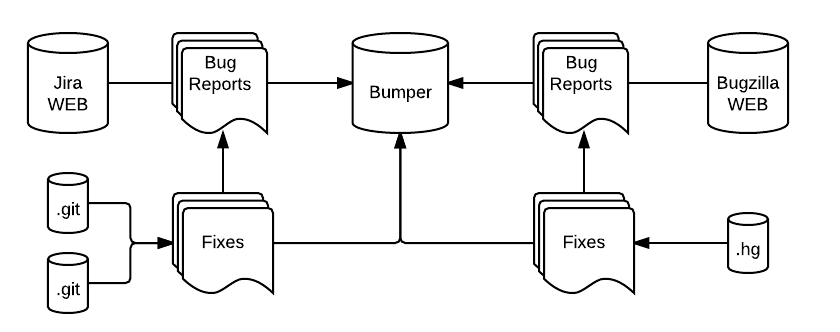
\includegraphics{media/bumper-approach.png}
    \caption{Overview of the bumper database construction.
    \label{fig:bumper-approach}}
\end{figure}

We used the same datasets presented earlier in Table \ref{table:datasets}.
We choose to use the same ones as these two datasets because they exposed a great diversity in programming languages, teams, localization, utility and maturity. Moreover, the used different tools, i.e. Bugzilla, JIRA, Git and Mercurial, and therefore, BUMPER is ready to host any other datasets that used any composition of these tools.

\section{Architecture}

{\tt BUMPER} rely on a highly scalable architecture composed of two distinct servers as depicted in Figure \ref{fig:bumper-arch}. The first server, on the left, handles the web requests and runs three distinct components:

\begin{itemize}
	\item Pound is a lightweight open source reverse proxy program and application firewall.
	It is also served us to decode  to request to http. Translating an  request to http and then, use this HTTP request instead of the  one allow us to save the http's decryption time required at each step.
	Pound also acts as a load-balancing service for the lower levels.
	\item Translated requests are then handled to Varnish. Varnish is an HTTP accelerator designed for content-heavy and dynamic websites. What it does is caching request that come in and serve the answer from the cache is the cache is still valid.
	\item NginX (pronounced engine-x) is a web-server that has been developed with a particular focus on high concurrency, high performances and low memory usage.
\end{itemize}

On the second server, that concretely handles our data, we have the following items:

\begin{itemize}
	\item Pound. Once again, we use pound here, for the exact same reasons.
	\item SolrCloud is the scalable version of Apache Solr where the data can be separated into shards (e.g chunk of manageable size). Each shard can be hosted on a different server, but it's still indexed in a central repository. Hence, we can guarantee a low query time while exponentially increasing the data.
	\item Lucene is the full text search engine powering Solr. Each Solr server has its own embedded engine.
\end{itemize}

\begin{figure}[h!]
  \centering
    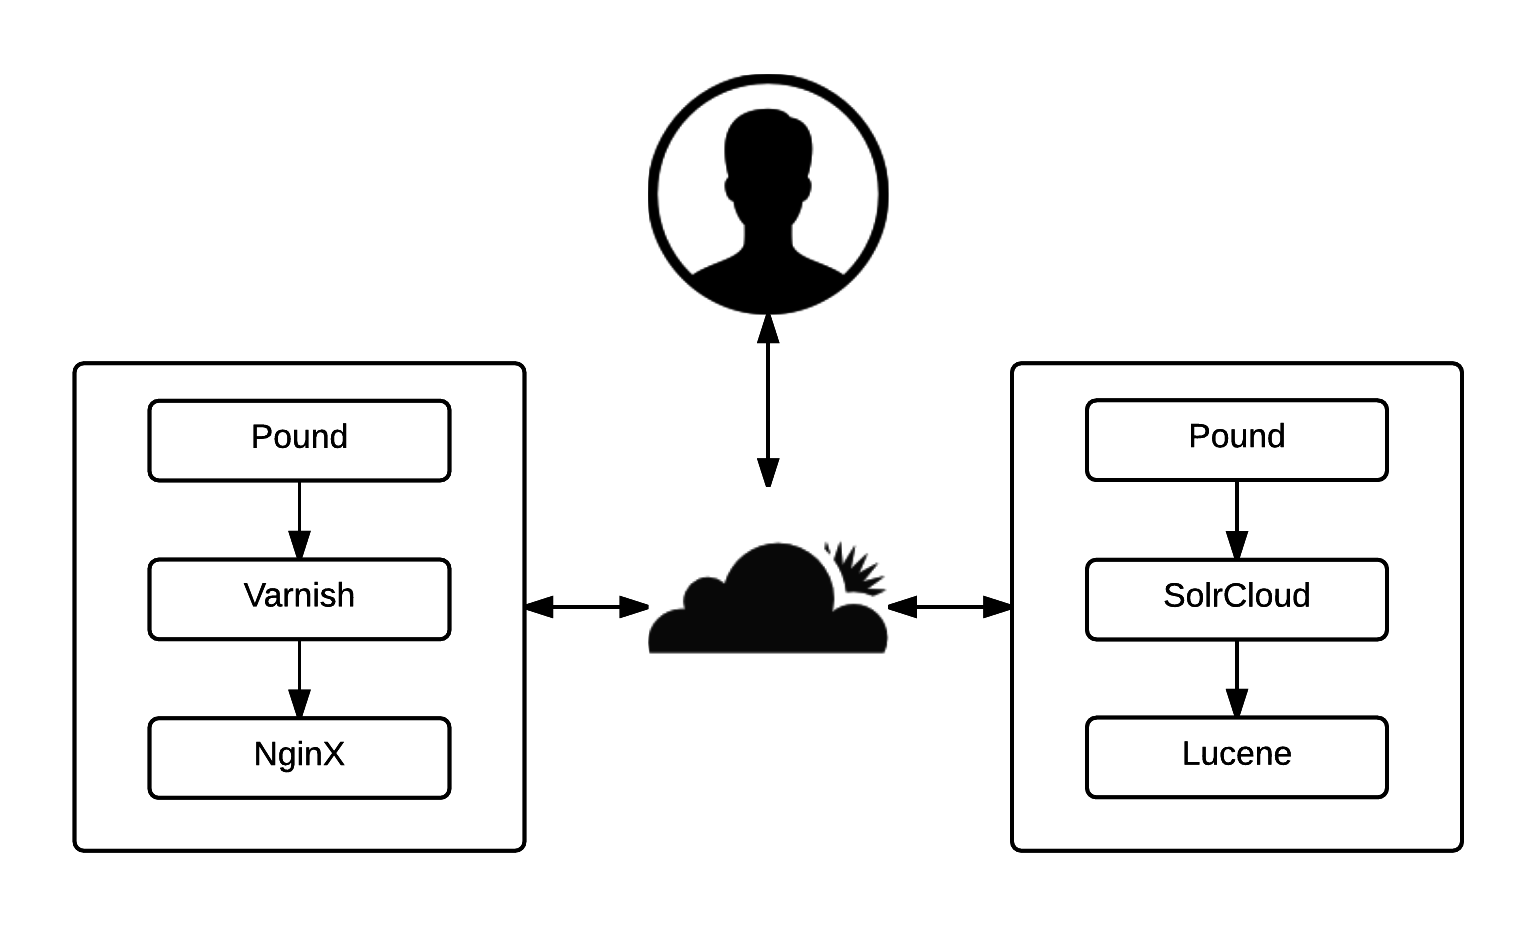
\includegraphics{media/bumper-arch.png}
    \caption{Overview of the bumper architecture.
    \label{fig:bumper-arch}}
\end{figure}

Request from users to the servers and the communication between our servers are going through the CloudFlare network.
CloudFlare acts as a content delivery network sitting between the users and the webserver.
They also provide an extra level of caching and security.

To give the reader a glimpse about the performances that this unusual architecture can yield; we are able to request and display the result of a specific request in less than 100 ms while our two servers are, in fact, two virtual machines sharing an AMD Opteron (tm) Processor 6386 SE (1 core @ 2,000 MHz) and 1 GB of RAM.

\section{UML Metamodel}

Figure \ref{fig:bumper-approach} presents the simplified {\tt BUMPER} metamodel that we designed according to our bug taxonomy presented in section \ref{fig:bug-taxo} and according to our future needs for {\tt JCHARMING}, {\tt RESSEMBLE} and {\tt BIANCA}.

\begin{figure}[h!]
  \centering
    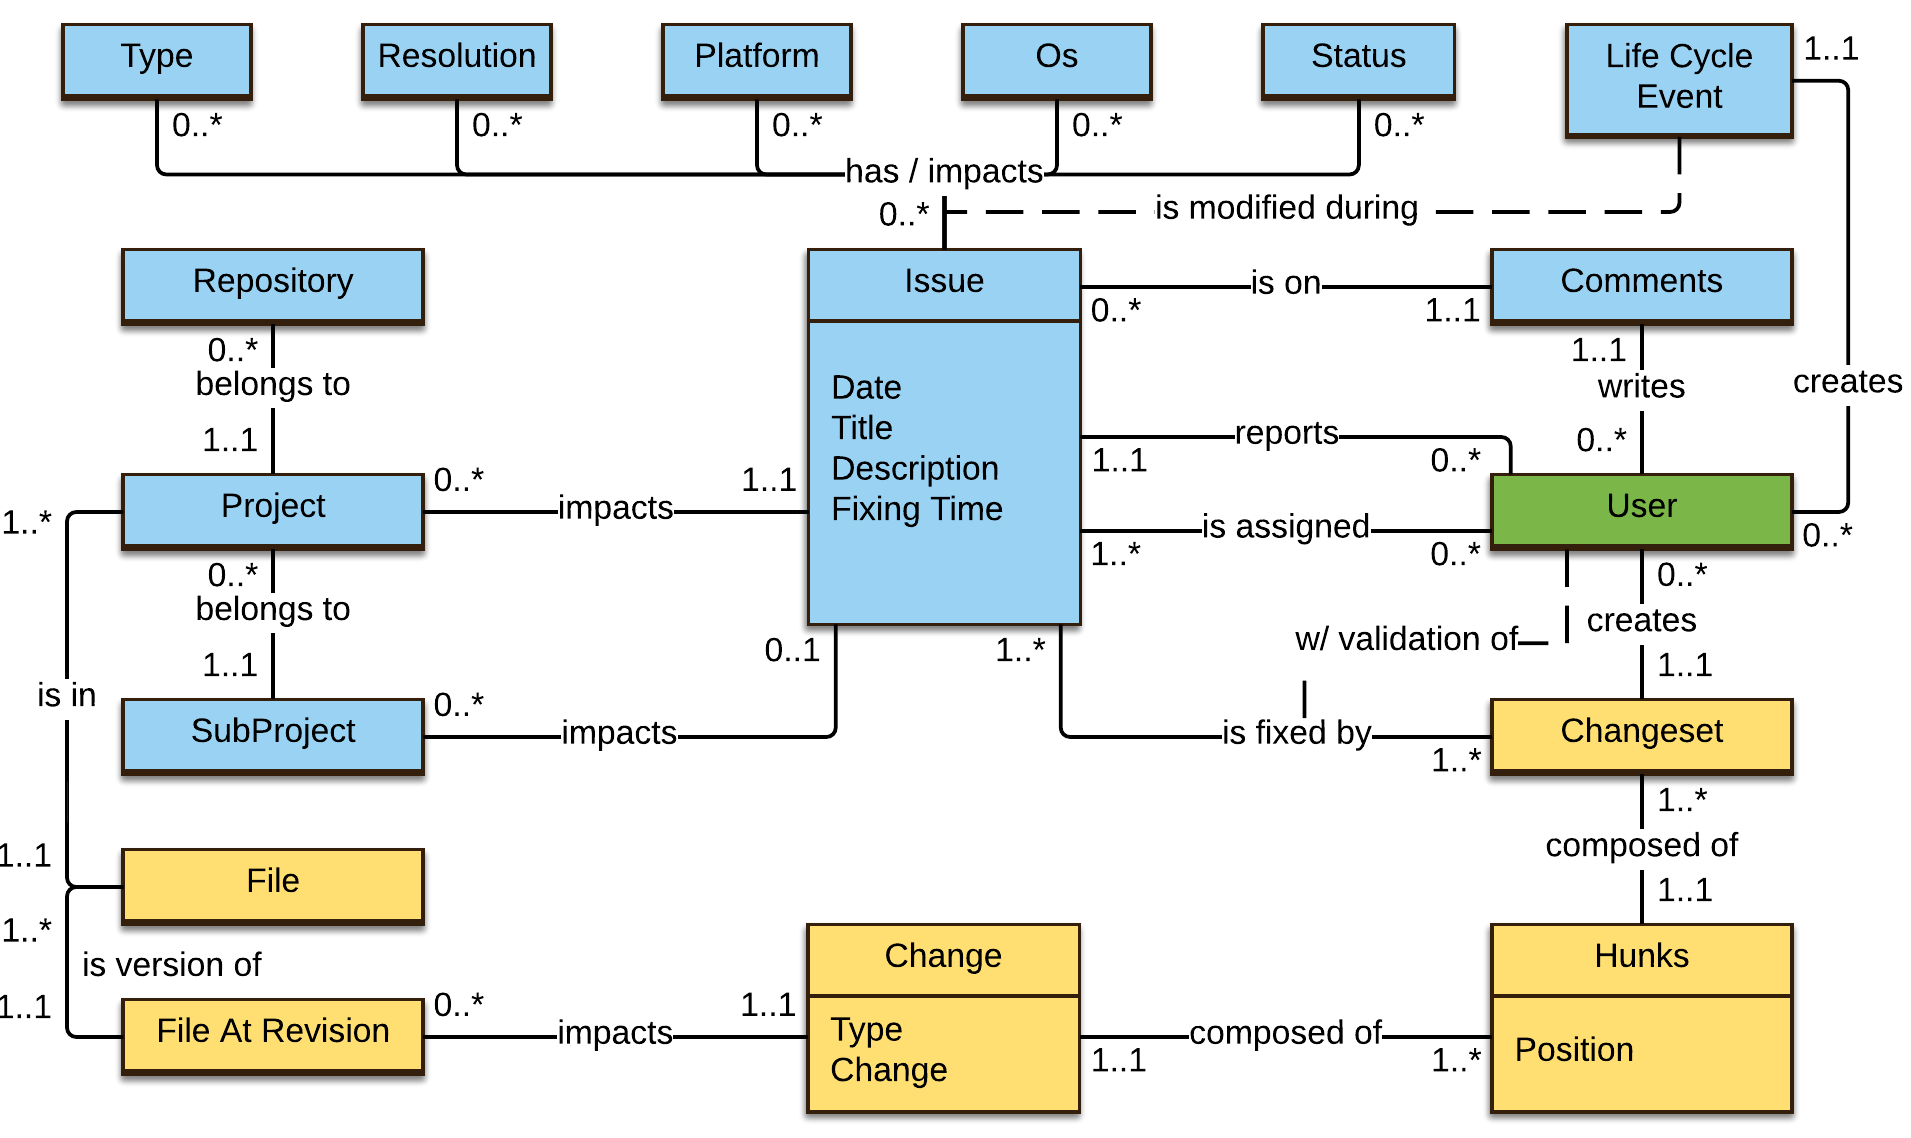
\includegraphics{media/bumper-model.png}
    \caption{Overview of the bumper meta-model.
    \label{fig:bumper-approach} }
\end{figure}


An {\it issue} ({\it task}) is characterized by a {\it date}, {\it title}, {\it description}, and a {\it fixing time}. They are reported (created) by and assigned to {\it users}.
Also, {\it issues} ({\it tasks}) belong to {\it project} that are in {\it repository} and might be composed of {\it sub-projects}.
{\it Users} can modify an {\it issue} ({\it task})  during {\it life cycle events} which impact the {\it type}, the {\it resolution}, the {\it platform}, the {\it OS} and the {\it status}. {\it Issues} ({\it tasks}) are resolved (implemented) by {\it changeset} that are composed of {\it hunks}. {\it Hunks} contain the actual changes to a {\it file} at a given revision, which are versions of the {\it file} entity that belongs to a {\it Project}.


\section{Features}

In this section, we present the features of bug report and their fixes in details.

\subsection{Bug Report}

A bug report is characterized by the following features:


\begin{itemize}

\item ID: unique string id of the form bug\_dataset\_project\_bug\_id
\item Dataset: the dataset of which the bug is extracted from.
\item Type: The type help us to distinguish different type of entities in BUMPER, i.e the bugs, changesets and hunks. For bug report, the type is always set to BUG
\item Date: The date at which the bug report has been submitted.
\item Title: The title of the bug report.
\item Project: The project that this bug affects.
\item Sub\_project: The sub-project that this bug affects.
\item Full\_name\_project: The combination of the project and the sub-project.
\item Version: the version of the project that this bug affects
\item Impacted\_platform: the platform that this bug affects
\item Impacted\_os: the operating system that this bug affects
\item Bug\_status: The status of the bug. As in bumper, our main concern is on the relationship between of fix and a bug, we only have RESOLVED bugs
\item Resolution: How the bug was resolved. Once again, as we are interested in investigating the fixes and the bugs, we only have FIXED bugs.
\item Reporter\_pseudo: the pseudonym of the person who report the bug.
\item Reporter\_name: the name of the person who reported the bug
\item Assigned\_to\_pseudo: the pseudonym of the person who have \item been assigned to fix this bug
\item Assigned\_to\_name: the name of the person who have been assigned to fix this bug
\item Bug\_severity: the severity of a bug
\item Description: the description of the bug the reporter gave
\item Fixing\_time: The time it took to fix the bug, i.e the elapsed time between the creation of the BR and its modification to resolve/fixed, in minutes
\item Comment\_nb: How many comments have been posted on the bug report system for that bug
\item Comment: Contains one comment. A bug can have 0 or many comments
\item File: A file qualified name that has been modified in order to fix a bug. A bug can have 0 (in case we did not find its related commit) or many files.

\end{itemize}

We selected this set of features for bug report as they are the ones that are analyzed in many past and recent studies. In addition, bugs can contain 0 or many .

\subsection{Changesets}

In this section, we present the features that characterize changeset entities in BUMPER.

\begin{itemize}

\item ID: the SHA1 hash
\item User: the name and email of the person who submitted that commit
\item Date: the date at which this commit has been fixed
\item Summary: the commit message entered by the user
\item File: The fully qualified name of a file modified on that commits. A changeset can have 1 or many files.
\item Number\_files: How many files have been modified in that commit
\item Insertions: the number of inserted lines
\item Deletions: the number of deleted lines
\item Churns: the number of modified lines
\item Hunks: the number of sets of consecutive changed lines
\item Parent\_bug: the id of the bug this changeset belongs to.

\end{itemize}

In addition, changesets contain one or many hunks.

\subsection{Hunks}
A hunks are a set of consecutive lines changed in a file in order. A set of hunks form a fix that can be scattered across one or many files. Knowing how many hunks a fixed required and what are the changes in each of them is useful, as explained by [2] to understand how many places developers have to go to fix a bug.

Hunks are composed of:

\begin{itemize}
\item ID: unique id based on the files, the insertion and the SHA1 of the commits
\item Parent\_changeset: the SHA1 of the Changeset this hunk belongs to
\item Parent\_bug: the id of the bug this hunk belongs to.
\item Negative\_churns: how many lines have been removed in that hunk
\item Positive\_churns: how many lines have been added in that hunk
\item Insertion: the position in a file at which this hunk takes place.
\item Change: One line that have been added or removed. A Hunk can contain one or many changes.
\end{itemize}

\section{Application Program Interface (API)\label{sec:bumper-api}}

BUMPER is available for engineers and researchers at {\bf https://bumper-app.com} and take the form of a regular search engine. Bumper supports (1) natural language query, (2) parent-child relationships, query, (3) disjunctions and union between complex queries and (4) a straight forward export of query results in XML, CSV or JSON format.

Browsing BUMPER, the basic query mode, perform the following operation:

\begin{equation}
\begin{split}
(type:BUG~AND~report\_t:(``YOUR~TERMS''))~OR~(!parent~which=type``BUG'')~\\fix\_t:``YOUR~TERMS'')
\end{split}
\end{equation}

The first part of the query component of the query retrieves all the bugs that contains the $``YOUR~TERMS''$ query in at least one its features by selecting type: BUG and report\_t, which is an index composed of all the features of the bug, set to $``YOUR~TERMS''$.
Then, we merge this query with another one that reads \\
$(!parent~which=type``BUG'')fix\_t:~``YOUR~TERMS'')$.
In this one, we retrieve the parent documents, i.e the bugs, of fixes that contains $``YOUR~TERMS''$ in their $fix\_t$ index.
The $fix\_t$ index is, as for the BUG, an index based on all the fields of changeset and hunk both. As a result, we search seamlessly in the bug report and their fixes in natural language.

As a more practical example, Figure \ref{fig:bumper-live} illustrate a query on https://bumper-app.com. The search term is  ``{\it Exception}'' and we can see that 20,285 issues / tasks have been found in 25 ms This particular set of issues, displayed on the left side, match because they contain ``{\it Exception}'' in the issue report or in the source code modified to fix this issue (implement this task). Then on the right side of the screen, the selected issue (task) is displayed. We can see the basic characteristic of the issue (task) followed by comments and finally, the source code.

\begin{figure}[h!]
  \centering
    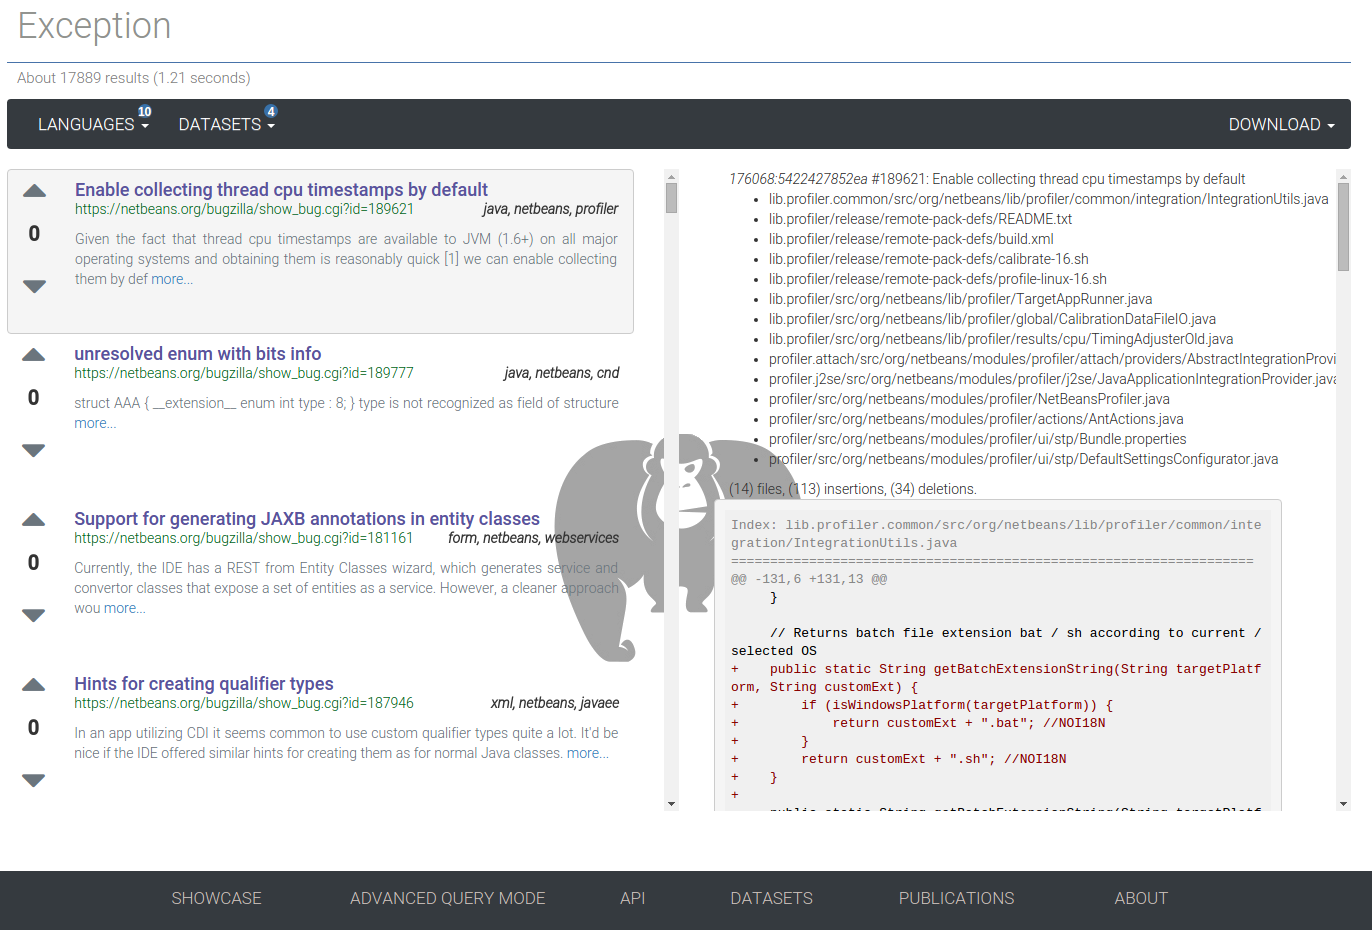
\includegraphics[scale=0.3]{media/bumper-live.png}
    \caption{Screenshot of https://bumper-app.com with ``Exception'' as research.
    \label{fig:bumper-live}}
\end{figure}


Moreover, BUMPER supports AND, OR, NOR operators and provide results in order of seconds.

As we said before, BUMPER is based on Apache Solr which have an incredibly rich API that is available online\footnote{ http://lucene.apache.org/solr/resources.html}.

{\tt BUMPER} serves as data repositories for the upcoming approaches presented in the chapters.


\chapter{JCHARMING: Java CrasH Automatic Reproduction by directed Model checkING\label{chap:jcharming}}

In this chapter, we present {\tt JCHARMING} (Java CrasH Automatic Reproduction by directed Model checkING).
{\tt JCHARMING} is an approach to reproduce field-crash.
Every time a bug report is submitted to a project management system and aggregated by {\tt BUMPER}, {\tt JCHARMING} will try to reproduce it.
In case of success, the steps to reproduce the bug are saved in {\tt BUMPER}.

The materials presented in this chapter are based on the following publications:

\begin{itemize}
	\item Nayrolles, M. , Hamou-Lhadj, W., Tahar, S. & Larsson, A. (2016). A Bug Reproduction Approach Based on Directed Model Checking and Crash Traces. Journal of Software: Evolution and Process. Wiley. 2016. (Accepted).
	\item Nayrolles, M. , Hamou-Lhadj, W., Tahar, S. & Larsson, A. JCHARMING : A Bug Reproduction Approach Using Crash Traces and Directed Model Checking. In Proceeding of the International Conference on Software Analysis, Evolution, and Reengineering (SANER'15), pages 101-110, 2015. (Best Paper Award).
\end{itemize}

%!TEX root = ../research_proposal.tex

\section{JCHARMING - Java CrasH Automatic Reproduction by directed Model checkING\label{sec:JCHARMING}}

Field failures are challenging to reproduce because
the data provided by the end users is often scarce. A survey
conducted with developers of major open source software
systems such as Apache, Mozilla and Eclipse revealed that
one of the most valuable piece of information that can help
locate and fix the cause of a crash is the one that can help
reproduce it \cite{Bettenburg2008}. It is therefore important to invest in
techniques and tools for automatic bug reproduction to ease
the maintenance process and accelerate the rate of bug fixes
and patches.

In this section, we present an approach, called {\tt JCHARMING}
(Java CrasH Automatic Reproduction by directed Model
checkING) that uses a combination of crash traces and model
checking to automatically reproduce bugs that caused field
failures. Unlike existing techniques, such as on-field record and in-house replay \cite{Narayanasamy2005,Artzi2008,Jaygarl} or crash explanation \cite{Manevich2004,chandra2009snugglebug} JCHARMING does not
require instrumentation of the code. It does not need access to
the content of the heap either. Instead, JCHARMING uses a
list of functions output when an uncaught exception in Java
occurs (i.e., the crash trace) to guide a model checking engine
to uncover the statements that caused the crash. While we do not filter any personal information that may appear in the crash trace, JCHARMING  raises less privacy concerns than a tool recording every call or dump the content of the memory.

To assess the effiency of {\tt JCHARMING} we try to reproduce issues contained in {\tt BUMPER}.

\subsection{Preliminaries}

Model checking (also known as property checking) will, given a system (that could be software \cite{Visser2003} or hardware based \cite{kropf1999introduction}), check if the system meets a specification Spec by testing exhaustively all the states of the system under test (SUT), which can be represented by a Kripke \cite{Kripke1963} structure:

\begin{equation}
SUT = <S,T,P>
\end{equation}

where S is the set of states, $T \subseteq S * S$ represents the transitions between the states and P is the set of properties that each state satisfies. The SUT is said to satisfy a set of properties p when there exists a sequence of states transition x leading towards these properties. This can be written as:

\begin{equation}
(SUT, x)  \models p
\end{equation}

However, this only ensures that $\exists x$ such that $p$ is reached at some point in the execution of the program and not that $p$ holds nor that $\forall x$, $p$ is satisfiable. In JCHARMING, SUTs are bound to a simple specification: they must not crash under a fair environment. In the framework of this study, we consider a fair environment as any environment where the transitions between the states represent the functionalities offered by the program. For example, in a fair environment, the program heap or other memory spaces cannot be modified. Without this fairness constraint, all programs could be tagged as buggy since we could, for example, destroy objects in memory while the program continues its execution. As we are interested in verifying the absence of unhandled exceptions in the SUT, we aim to verify that for all possible combinations of states and transitions there is no path leading towards a crash. That is:

\begin{equation}
\forall x.(SUT, x) \models \neg c
\end{equation}

If such a path exists (i.e., $\exists x$  such that $(SUT, x)  \models c$) then the model checker engine will output the path $x$ (known as the counter-example) which can then be executed. The resulting Java exception crash trace is compared with the original crash trace to assess if the bug is reproduced. While  being  accurate and exhaustive in finding counter-examples, model checking suffers from the state explosion problem, which hinders its applicability to large software systems.


To show the contrast between testing and model checking, we use the hypothetical example of Figures \ref{fig:testing-toy}, \ref{fig:checking-toy} and \ref{fig:dchecking-toy} to sketch the possible results of each approach. These figures depicts a toy program where from the entry point, unknown calls are made (dotted points) and, at some points, two methods are called. These methods, called \texttt{Foo.Bar} and \texttt{Bar.Foo}, implement a for \texttt{loop} from 0 to \texttt{loopCount}. The only difference between these two methods is that the \texttt{Bar.Foo} method throws an exception if i becomes larger than two. Hereafter, we denote this property as $c_{i > 2}$.  


\begin{figure}[h!]
  \centering
    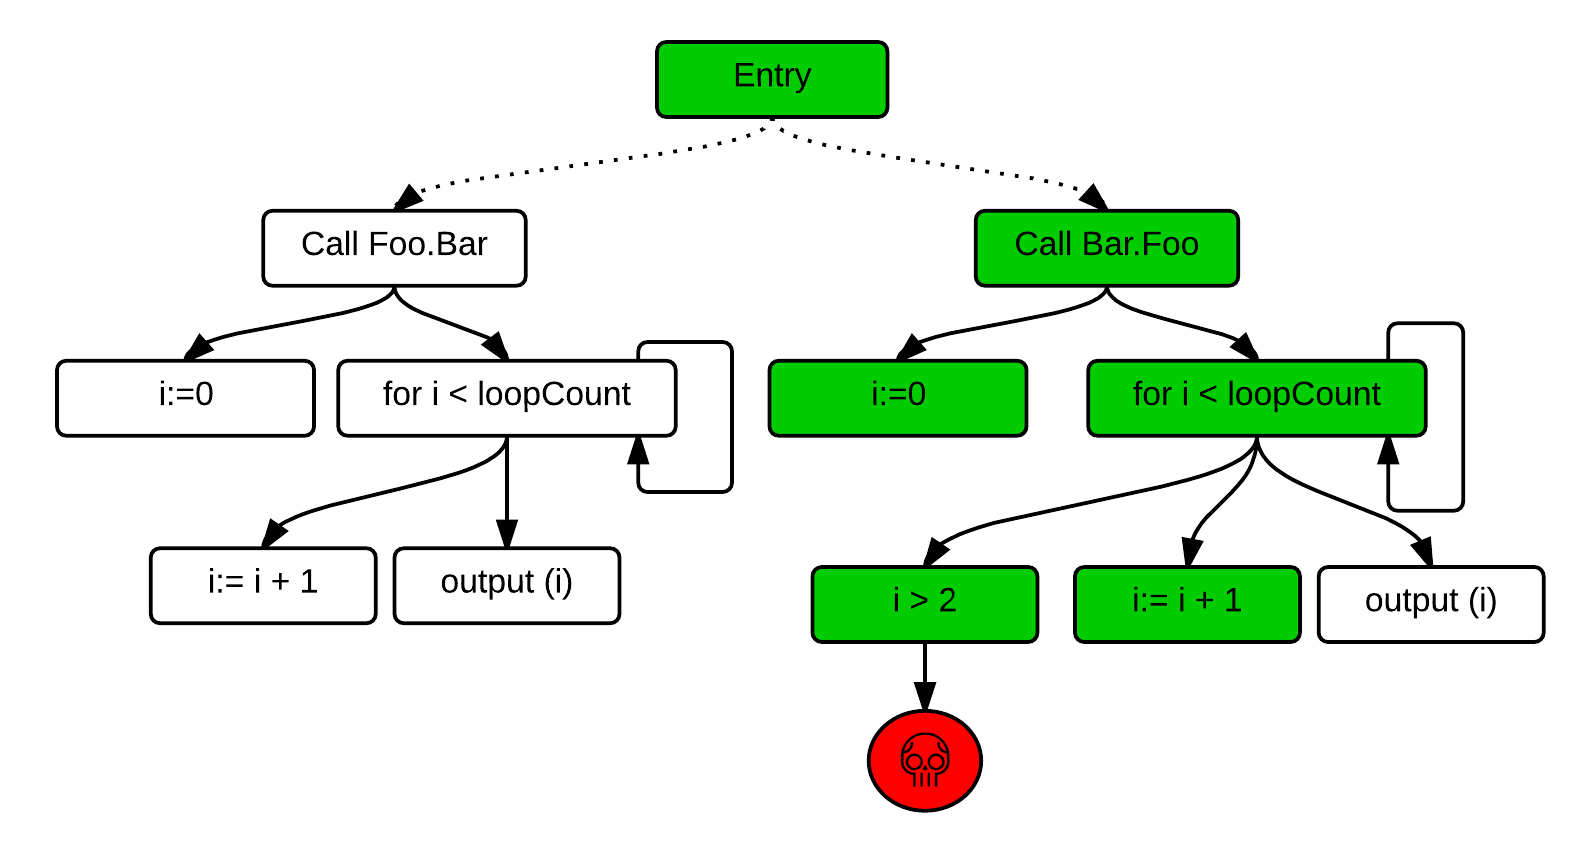
\includegraphics{media/dmc.png}
    \caption{A toy program under testing
    \label{fig:testing-toy}}
\end{figure}

\begin{figure}[h!]
  \centering
    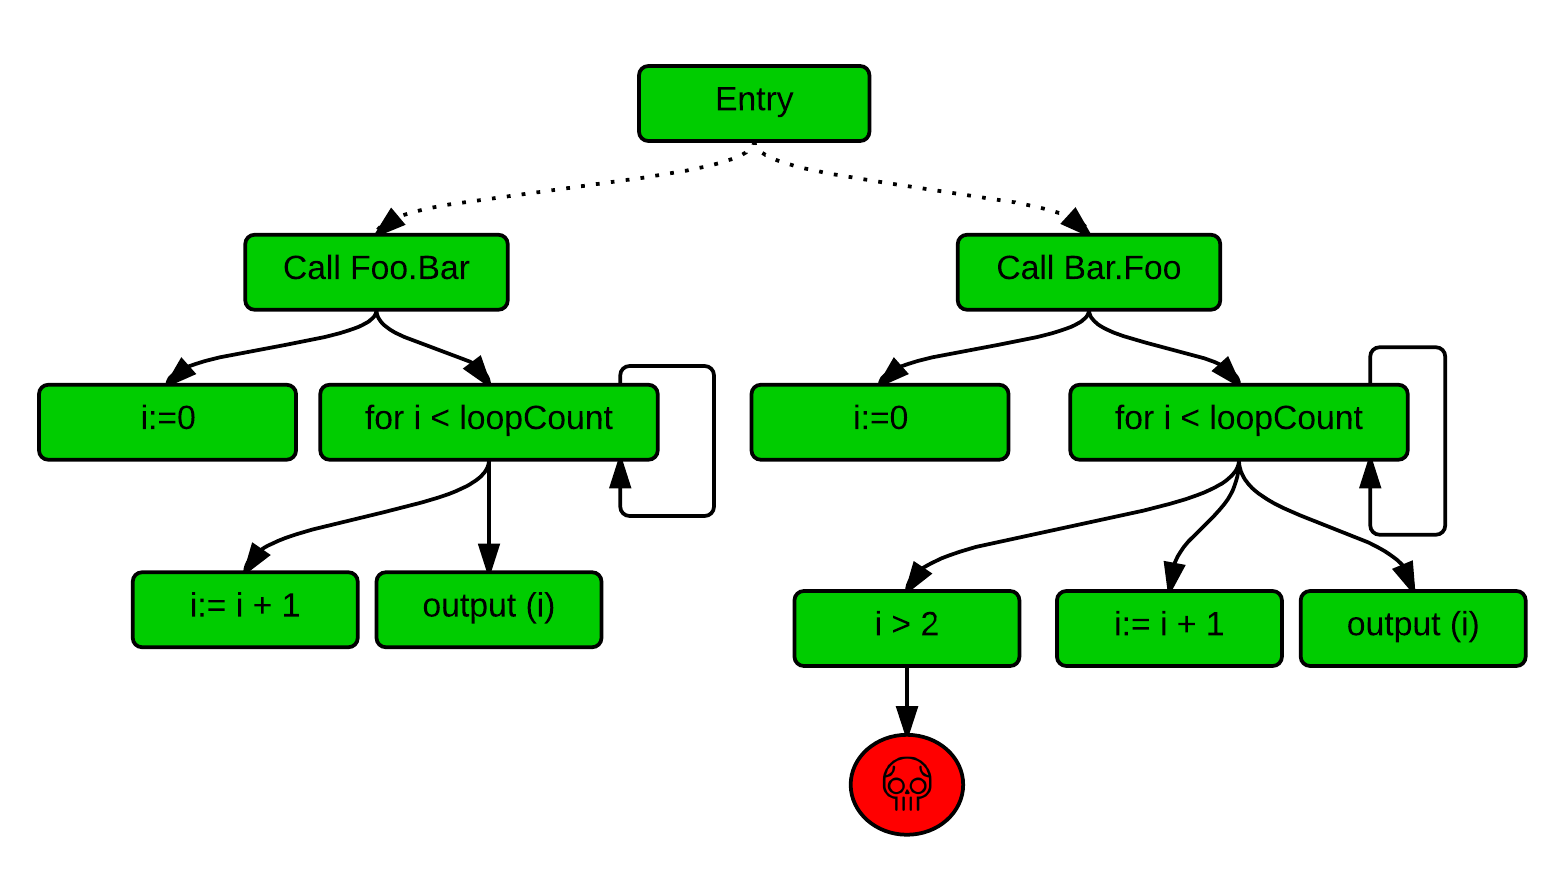
\includegraphics{media/mc.png}
    \caption{A toy program under model checking
    \label{fig:checking-toy}}
\end{figure}

\begin{figure}[h!]
  \centering
    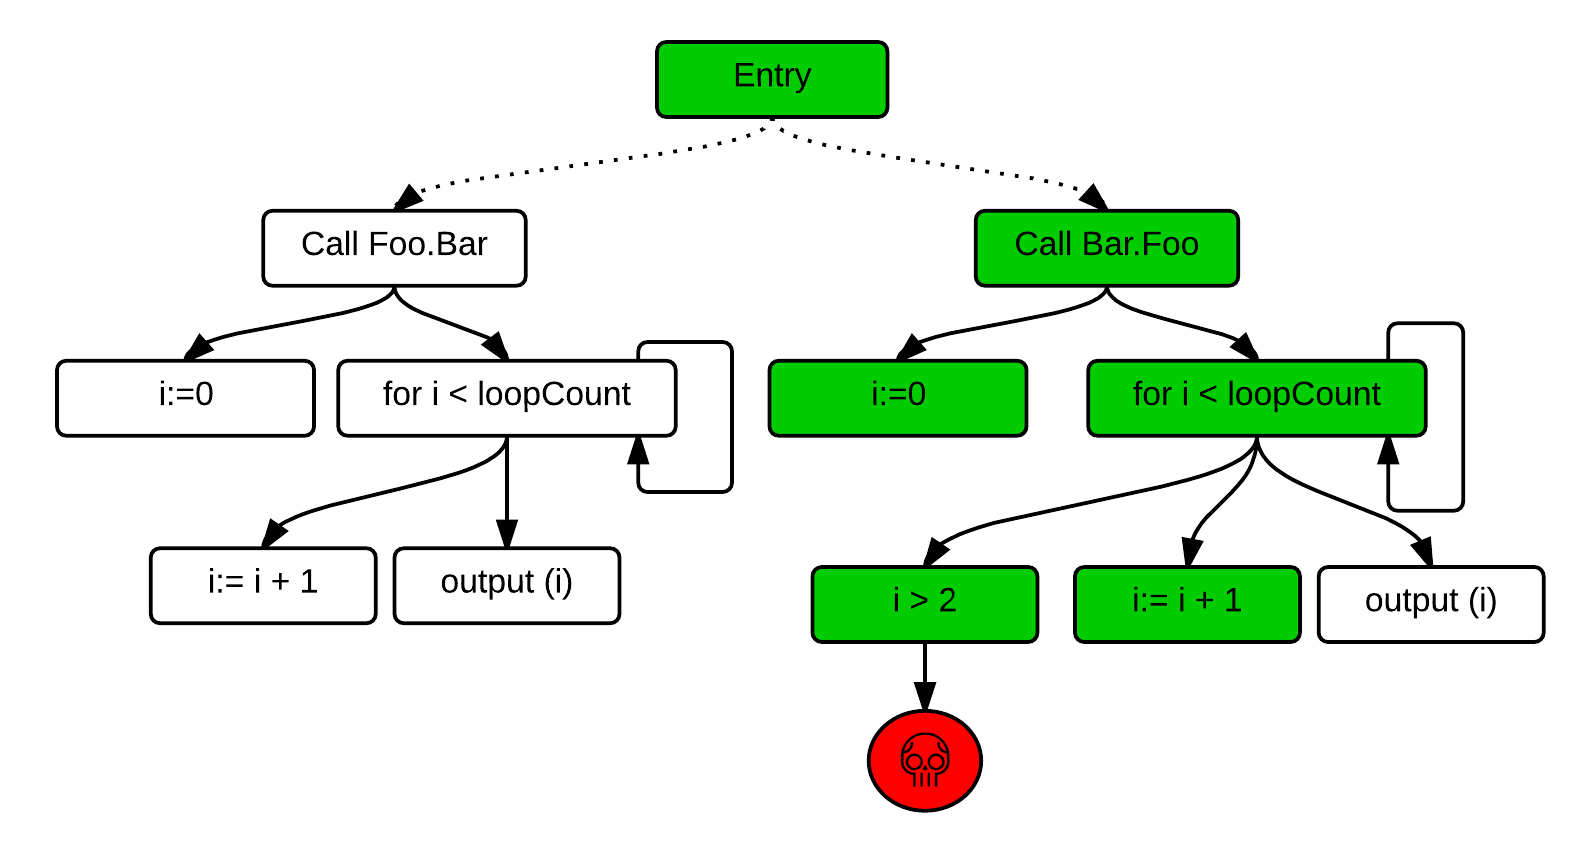
\includegraphics{media/dmc.png}
    \caption{A toy program under directed model checking
    \label{fig:dchecking-toy}}
\end{figure}

Figure \ref{fig:testing-toy} shows the program statements that could be covered using testing approaches. Testing software is a demanding task where a set of techniques is used to test the SUT according to some input.

Software testing depends on how well the tester understands the SUT in order to write relevant test cases that are likely to find errors in the program. Program testing is usually insufficient because it is not exhaustive. In our case, using testing would mean that the tester knows what to look for in order to detect the causes of the failure. We do not assume this knowledge in JCHARMING. 

Model checking, on the other hand, explores each and every state of the program (Figure \ref{fig:checking-toy}), which makes it complete, but impractical for real-world and large systems. To overcome the state explosion problem of model checking, directed (or guided) model checking has been introduced \cite{Rungta2009}. Directed model checking use insights—generally heuristics—about the SUT in order to reduce the number of states that need to be examined. Figure \ref{fig:dchecking-toy} explores only the states that may lead to a specific location, in our case, the location of the fault. The challenge, however, is to design techniques that can guide the model checking engine. As we will describe in the next section, we use crash traces and program slicing to overcome this challenge.

\subsection{The JCHARMING Approach}

Figure \ref{fig:jcarming-approach} shows an overview of JCHARMING. The first step
consists of collecting crash traces, which contain raw lines
displayed to the standard output when an uncaught exception
in Java occurs. In the second step, the crash traces are
preprocessed by removing noise (mainly calls to Java standard
library methods). The next step is to apply backward slicing
using static analysis to expand the information contained in
the crash trace while reducing the search space. The resulting
slice along with the crash trace are given as input to the model
checking engine. The model checker executes statements
along the paths from the main function to the first line of the
crash trace (i.e., the last method executed at crash time, also
called the crash location point). Once the model checker finds
inconsistencies in the program leading to a crash, we take the
crash stack generated by the model checker and compare it to
the original crash trace (after preprocessing). The last step is
to build a JUnit test, to be used by software engineers to
reproduce the bug in a deterministic way.

\begin{figure}[h!]
  \centering
    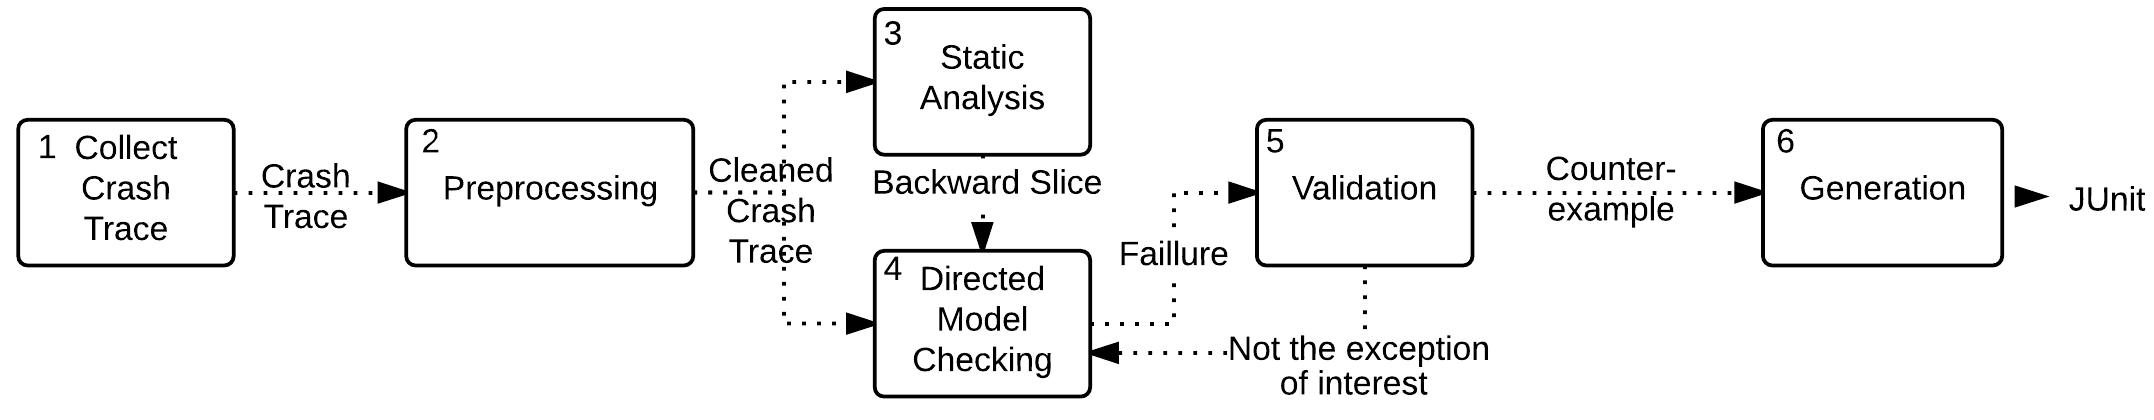
\includegraphics[scale=0.8]{media/jcharming-approach.png}
    \caption{Overview of JCHARMING.
    \label{fig:jcarming-approach}}
\end{figure}

\subsubsection{Collecting Crash Traces}

The first step of JCHARMING is to collect the crash trace
caused by an uncaught exception. Crash traces are usually included in crash reports and can therefore be automatically
retrieved using a simple regular expression.
Figure \ref{fig:jcarming-traces} shows an example of a crash trace that contains the
exception thrown when executing the program depicted in
Figures \ref{fig:testing-toy} to \ref{fig:dchecking-toy}. The crash trace contains a call to the Bar.foo()
method—the crash location point—and calls to Java standard
library functions (in this case, GUI methods because the
program was launched using a GUI).

\begin{figure}[h!]
  \noindent\fbox{%
      \parbox{\textwidth}{%
  1.javax.activity.InvalidActivityException:loopTimes \\
  should be < 3 \\
  2. at Foo.bar(Foo.java:10) \\
  3. at GUI.buttonActionPerformed(GUI.java:88) \\
  4. at GUI.access$0(GUI.java:85) \\
  5. at GUI$1.actionPerformed(GUI.java:57) \\
  6. caused by java.lang.IndexOutOfBoundsException : 3 \\
  7. at scam.Foo.buggy(Foo.java:17) \\
  8. and 4 more ...
      }%
  }
    \caption{Java InvalidActivityException is thrown in the Bar.Goo loop if the control variable is greater than 2.
    \label{fig:jcarming-traces}}
\end{figure}

As shown in Figure \ref{fig:jcarming-traces}, we can see that the first line (referred to
as frame {\it $f_0$} , subsequently the next line is called frame {\it $f_1$} , etc.)
does not represent the real crash point but it is only the last
exception of a chain of exceptions. Indeed, the {\tt InvalidActivity}
has been triggered by an {\tt IndexOutOfBoundsException} in
{\tt scam.Foo.buggy} . This kind of crash traces reflects several
nested try/catch blocks.

In addition, it is common in Java to have incomplete crash
traces. According to the Java documentation \cite{Oracle2011}, line 8 of
Figure \ref{fig:jcarming-traces} should be interpreted as follows: {\it ``This line indicates
that the remainder of the stack trace for this exception
matches the indicated number of frames from the bottom of the
stack trace of the exception that was caused by this exception
(the ``enclosing exception''). This shorthand can greatly
reduce the length of the output in the common case where a
wrapped exception is thrown from the same method as the
``causative exception'' is caught.}''

We are likely to find shortened traces in bug repositories as
they are what the user sees without any possibility to expand
their content.

\subsubsection{Preprocessing}

In the preprocessing step, we first reconstruct and reorganize
the crash trace in order to address the problem of nested
exceptions. Then, with the aim to obtain an optimal guidancefor our directed model checking engine, we remove frames
that are out of our control. Frames out of our controls refer
usually, but are not limited to, Java library methods and third
party libraries. In Figure \ref{fig:jcarming-traces}, we can see that Java GUI and
event management components appear in the crash trace. We
assume that these methods are not the cause of the crash;
otherwise it means that there is something wrong with the on-
field JDK. If this is the case, we will not be able to reproduce
the crash. Note that removing these unneeded frames will also
reduce the search space of the model checker.

\subsubsection{Building the Backward Static Slice}

For large systems, a crash trace does not necessary contain all
the methods that have been executed starting from the entry
point of the program (i.e., the main function) to the crash
location point. We need to complete the content of the crash
trace by identifying all the statements that have been executed
starting from the main function until the last line of the
preprocessed crash trace. In Figure \ref{fig:jcarming-traces}, this will be the function
call {\tt Bar.foo()}, which happens to be also the crash location
point. To achieve this, we turn to static analysis by extracting
a backward slice from the main function of the program to the
{\tt Bar.foo()} method.

A backward slice contains all possible branches that may lead
to a point {\it n} from a point {\it m} as well as the definition of the
variables that control these branches \cite{de2001program}. In other words, the
slice of a program point {\it n} is the program subset that may
influence the reachability of point {\it n} starting from point {\it m}.
The backward slice containing the branches and the definition
of the variables leading to {\it n} from {\it m} is noted as {\it $bslice_{[m \leftarrow n]}$}.

We perform a static backward slice between each frame to
compensate for possible missing information in the crash
trace. More formally, the final static backward slice is
represented as follows:

\begin{equation}
\centering
\begin{split}
bslice_{[entry \leftarrow f_0]} = bslice_{[f_1 \leftarrow f_0]} \cup bslice_{[f_2 \leftarrow f_1]} \cup ... \cup bslice_{[f_n \leftarrow f_{n−1}]} \cup bslice_{[entry \leftarrow f_n]}
\end{split}
\end{equation}

Note that the union of the slices computed between each pair
of frames must be a subset of the final slice between $f_0$ and the
entry point of the program. More formally:

\begin{equation}
\centering
\begin{split}
\bigcup_{i=0}^{entry} bslice_{[f_{i+1} \leftarrow f_i]} \subseteq bslice_{[entry \leftarrow f_0]}
\end{split}
\end{equation}

Indeed, in Figure \ref{fig:jcharming-slice}, the set of states allowing to reach $f_0$ from
$f_2$ is greater than the set of states to reach $f_1$ from $f_2$ plus set
of states to reach $f_0$ from $f_1$ . In this hypothetical example and
assuming that $z_2$ is a prerequisite to $f_2$ then
$bslice_{[entry \leftarrow f_0]} = \{f_0 , f_1 , f_2 , z_0 , z_1 , z_2 , z_3 \}$
while $\cup_{i=0}^n bslice_{[f_{i+1} \leftarrow f_i]}$.

\begin{figure}[h!]
  \centering
    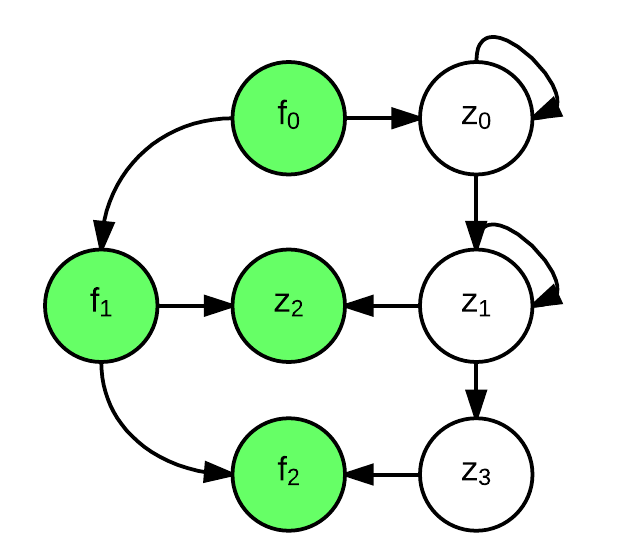
\includegraphics{media/jcharming-slices.png}
    \caption{Hypothetical example representing $bslice_{[entry \leftarrow f_0]}$ Vs. $\cup_{i=0}^n bslice_{[f_{i+1} \leftarrow f_i]} = \{f_0 , f_1 , f_2 , z_2 \}$
    \label{fig:jcharming-slice}}
\end{figure}

In the worst case scenerio where there exists one and only one
transition between each frame, which is very unlikely for real
and complex systems, then $bslice_{[entry \leftarrow f_0]}$ and
 $\cup_{i=0}^n bslice_{[f_{i+1} \leftarrow f_i]}$ yield the same set of states with a
comparable computational cost since the number of branches
to explore will be the same in both cases.

Algorithm \ref{alg:jcharming-slice} is a high level
representation of how we compute the backward slice between
each frame. The algorithm takes as input the pre-processed
call trace, the byte code of the SUT, and the entry point. From
line 1 to line 5, we initialize the different variables used by the
algorithm. The main loop of the algorithm begins at line 6 and
ends at line 15. In this loop, we compute the static slice
between the current frame and the next one. If the computed
static slice is not empty then we update the final backward
slice with the newly computed slice.


\begin{algorithm}[H]
 \KwData{Crash Stack, BCode, Entry Point}
 \KwResult{BSolve}
 $Frames~frames~\leftarrow~extract~frames~from~crash~stack$\;
 Int n $\leftarrow$ size of frame\;
 Int offset $\leftarrow$ 1\;
 Bslice bSlice $\leftarrow$ $\emptyset$\;
\For{i $\leftarrow$ 0 to i $<$ n \&\& offset $<$ n - 1}{
  BSlice currentBSlice $\leftarrow$ backward slice from frames[i] to i + offset\;
  \eIf{currentBSlice $\not=$ $\emptyset$}{
   bSlice $\leftarrow$ bSlice $\cup$ currentBSlice\;
   offset $\leftarrow$ 1\;
  }{
   offset $\leftarrow$ offset +1\;
  }
}
\caption{High level algorithm computing the union of the slices\label{alg:jcharming-slice}}
\end{algorithm}

Using backward slicing, the search space of the model checker
that processes the example of Figures \ref{fig:testing-toy} to \ref{fig:dchecking-toy} is given by the
following expression:

\begin{equation}
  \exists x.
  \begin{pmatrix}
    \bigcup_{i=0}^{entry} bslice_{[f_{i+1} \leftarrow f_i]}  \subset SUT \\
    x.\bigcup_{i=0}^{entry} bslice_{[f_{i+1} \leftarrow f_i]}  \subset x.SUT
  \end{pmatrix}
  \models c_{i>2}
\end{equation}

That is, there exists a sequence of states transitions $x$ that
satisfies $c_{i>2}$ where both the transitions and the states are
entry
elements of $\bigcup_{i=0}^{entry} bslice_{[f_{i+1} \leftarrow f_i]}$ . Obviously, $c_{i>2}$ also
needs to be included for the final static slice to be usable by
the model checking engine. Consequently, the only frame that
need to be untouched for the backward static slice to be
meaningful is $f_0$.

\subsubsection{Directed Model Checking}

The model checking engine we use in this paper is called JPF
(Java PathFinder) \cite{Visser2004}, which is an extensible JVM for Java
bytecode verification. This tool was first created as a front-end
for the SPIN model checker \cite{holzmann1997model} in 1999 before being open-
sourced in 2005. JPF is organized around five simple
operations: (i) {\it generate states}, (ii) {\it forward}, (iii) {\it backtrack},
(iv) {\it restore state} and (v) {\it check}. In the forward operation, the
model checking engine generates the next state $s_{t+1}$ . If
$s_{t+1}$ has successors then it is saved in a backtrack table to be
restored later. The backtrack operation consists of restoring
the last state in the backtrack table. The restore operation
allows restoring any state and can be used to restore the entire
program as it was the last time we choose between two
branches. After each, forward, backtrack and restore state
operation the check properties operation is triggered.

In order to direct JPF, we have to modify the {\it generate states}
and the {\it forward} steps. The {\it generate states} is populated with
entry
the states in $\bigcup_{i=0}^{entry} bslice_{[f_{i+1} \leftarrow f_i]}  \subset SUT$ and we adjust the
{\it forward step} to explore a state if the target state $s_i+1$ and the
transition $x$ to pass from the current state $s_i$ to $s_{i+1}$ are in
$\bigcup_{i=0}^{entry} bslice_{[f_{i+1} \leftarrow f_i]}  \subset SUT$ and $x.\bigcup_{i=0}^{entry} bslice_{[f_{i+1} \leftarrow f_i]}  \subset x.SUT$.

\subsubsection{Validation}

To validate the result of directed model checking, we modify
the {\it check properties} step that checks if the current sequence
of states transitions $x$ satisfies a set a property. If the current
states transitions $x$ can throw an exception, we execute $x$ and
compare the exception thrown to the original crash trace (after
preprocessing). If the two exceptions match, we conclude that
the conditions needed to trigger the failure have been met and
the bug is reproduced.

However, as argued by Kim et al. in \cite{Kim2013b}, the same failure can
be reached from different paths of the program. Although the
states executed to reach the defect are not exactly the same,
they might be useful to enhance the understanding of the bug
by software developers, and speed up the deployment of a fix.
Therefore, in this paper, we consider a defect to be partially
reproduced if the crash trace generated from the model
checker matches the original crash trace by a factor of $t$, where
$t$ is a threshold specified by the user. $t$ is the percentage of
identical frames between both crash traces.

\subsubsection{Generating Test Cases for Bug Reproduction}

To help software developers reproduce the crash in a lab
environment we automatically produce the JUnit test cases
necessary to run the SUT to cause the exercise of the bug.

To build a test suite that reproduces a defect, we need to create
a set of objects used as arguments for the methods that will
enable us to travel from the entry point of the program to the
defect location. JPF has the ability to keep track of what
happens during model checking in the form of traces
containing the visited states and the value of the variables. We
leverage this capability to create the required objects and call
the methods leading to the failure location. Although we can
track back the internal state of objects at a specific time using
JPF, it can be too computationally taxing to recreate only the
objects needed to generate the bug. To overcome this, we use
serialization techniques \cite{Opyrchal1999}. We take advantage of features
offered by the XStream \cite{Xstream2011} library which enables the
serialization and deserialization of any Java object — even
objects that do not implement the Java Serializable interface.
We use the serialization when the model checker engine
performs too many operations modifying the property of a
given object. In such case, we serialize the last state of the
object.

\subsection{Case studies}

In this section, we show the effectiveness of JCHARMING to
reproduce bugs in seven open source systems\footnote{The bug reports used in this study and the result of the model checker are
made available for download from research.mathieu-
nayrolles.com/jcharming/} . The aim of the
case study is to answer the following question: {\it Can we use
crash traces and directed model checking to reproduce on-
field bugs in a reasonable amount of time?}

\subsubsection{Targeted Systems}

Table \ref{tab:jacharming-systems} shows the systems and their characteristics in terms of
Kilo Line of Code (KLoC) and Number of Classes (NoC).

\begin{table}[h!]
\centering
\begin{tabular}{c|c|c|c}
SUT        & KLOC & NoC  & Bug \#ID                                        \\ \hline \hline
Ant        & 265  & 1233 & 38622, 41422                                    \\
ArgoUML    & 58   & 1922 & 2603, 2558, 311, 1786                           \\
dnsjava    & 33   & 182  & 38                                              \\
jfreechart & 310  & 990  & 434, 664, 916                                   \\
Log4j      & 70   & 363  & 11570, 40212, 41186, 45335, 46271, 47912, 47957 \\
MCT        & 203  & 1267 & 440ed48                                         \\
pdfbox     & 201  & 957  & 1412, 1359 \\ \hline \hline
\end{tabular}
\caption{List of taget systems in terms of Kilo line of code (KLoC), number of classes (NoC) and Bug \# ID}
\label{tab:jacharming-systems}
\end{table}

Apache Ant \cite{ApacheSoftwareFoundation} is a popular command-line tool to build
make files. While it is mainly known for Java applications,
Apache Ant also allows building C and C++ applications. We
choose to analyze Apache Ant because it has been used by
other researchers in similar studies.

ArgoUML \cite{CollabNet} is one of the major players in the open source
UML modeling tools. It has many years of bug management
and, similar to Apache Ant, it has been extensively used as a
test subject in many studies.

Dnsjava \cite{Wellington2013} is a tool for the implementation of the DNS
mechanisms in Java. This tool can be used for queries, zone
transfers, and dynamic updates. It is not as large as the other
two, but it still makes an interesting case subject because it has
been well maintained for the past decade. Also, this tool is
used in many other popular tools such as Aspirin, Muffin and
Scarab.

JfreeChart \cite{ObjectRefineryLimited2005} is a well-known library that enables the
creation of professional charts. Similar to dnsjava, it has been
maintained over a very long period of time —JfreeChart was
created in 2005— and it is a relatively large application.

Apache Log4j \cite{TheApacheSoftwareFoundation1999} is a logging library for Java. This is not a
very large library, but it is extensively used by thousands of
programs. As other Apache projects, this tool is well
maintained by a strong open source community and allows
developers to submit bugs. The bugs which are in the bug
report system of Log4j are, generally speaking, well
documented and almost every bug contains a related crash
trace and, therefore, it is a tool of interest to us.

MCT \cite{NASA2009} stands for Mission Control technologies and was
developed by the NASA Ames Research Center (the creators
of JPF) for use in spaceflight mission operation. This tool
benefits from two years of history and targets a very critical
domain, Spacial Mission Control. Therefore, this tool has to
be particularly and carefully tested and, consequently, the
remaining bugs should be hard to discover and reproduce.

PDFBox \cite{ApacheSoftwareFoundation2014} is another tool supported by the Apache
Software Foundation since 2009 and was created in 2008.
PDFBox allows the creation of new PDF documents and the
manipulation of existing documents.

\subsubsection{Bug Selection and Crash Traces}

In this study, we have selected the reproduced bugs randomly
in order to avoid the introduction of any bias. We selected a
random number of bugs ranging from 1 to 10 for each SUT
containing the word ``exception'' and where the description of
the bug contains a match a regular expression designed to find the pattern of a
Java exception.

\subsection{Results}

Table \ref{tab:jcharming-results} shows the results of JCHARMING in terms of Bug
\#ID, reproduction status, and execution time (in minutes) of
directed model checking (DMC) and Model Checking (MC).
The experiments have been conducted on a Linux machine (8
GB of RAM and using Java 1.7.0\_51).

\begin{itemize}
  \item The result is noted as ``Yes'' if the bug has been fully
reproduced, meaning that the crash trace generated by the
model checker is identical to the crash trace collected
during the failure of the system.
\item The result is ``Partial'' if the similarity between the crash
trace generated by the model checker and the original
crash trace is above t=80\%. Given an 80\% similarity
threshold, we consider partial reproduction as successful.
A different threshold could be used.
\item Finally, the result of the approach is reported as ``No'' if
either the similarity is below t < 80\% or the model
checker failed to crash the system given the input we
provided.
\end{itemize}

\begin{table}[h!]
\centering
\begin{tabular}{c|c|c|c|c}
SUT                         & Bug \#ID & Reprod. & Time DMC & Time MC \\ \hline \hline
\multirow{2}{*}{Ant}        & 38622    & Yes     & 25.4     & -       \\
                            & 41422    & No      & -        & -       \\ \hline
\multirow{4}{*}{ArgoUML}    & 2558     & Partial & 10.6     & -       \\
                            & 2603     & Partial & 9.4      & -       \\
                            & 311      & Yes     & 11.3     & -       \\
                            & 1786     & Partial & 9.9      & -       \\  \hline
DnsJava                     & 38       & Yes     & 4        & 23      \\ \hline
\multirow{3}{*}{jFreeChart} & 434      & Yes     & 27.3     & -       \\
                            & 664      & Partial & 31.2     & -       \\
                            & 916      & Yes     & 26.4     & -       \\ \hline
\multirow{7}{*}{Log4j}      & 11570    & Yes     & 12.1     & -       \\
                            & 40212    & Yes     & 15.8     & -       \\
                            & 41186    & Partial & 16.7     & -       \\
                            & 45335    & No      & -        & -       \\
                            & 46271    & Yes     & 13.9    & -       \\
                            & 47912    & Yes     & 12.3     & -       \\
                            & 47957    & No      & -        & -       \\
MCT                         & 440ed48  & Yes     & 18.6     & -       \\ \hline
\multirow{2}{*}{PDFBox}     & 1412     & Partial & 19.7     & -       \\
                            & 1359     & No      & -        & - \\ \hline \hline
\end{tabular}

\caption{Effectiveness of JCHARMING using directed model checking (DMC) and model checking (MC) in minutes}
\label{tab:jcharming-results}
\end{table}

As we can see in Table \ref{tab:jcharming-results}, we were able to reproduce 17 bugs
out of 20 bugs either completely or partially (85% success
ratio). The average time to reproduce a bug is 16 minutes.
This result demonstrates the effectiveness of our approach,
more particularly, the use of backward slicing to create a
manageable search space that guides adequately the model
checking engine. We also believe that our approach is usable
in practice since it is also time efficient. Among the 20 different bugs we have tested, we will describe
one bug (chosen randomly) for each category (successfully
reproduced, partially reproduced, and not reproduced) for
further analysis.

\subsubsection{Successfully reproduced}

The first bug we describe in this discussion is the bug \#311
belonging to ArgoUML. This bug was submitted in an earlier
version of ArgoUML. This bug is very simple to manually
reproduce thanks to the extensive description provided by the
reporter, which reads: {\it ``I open my first project (Untitled Model by default). I choose
to draw a Class Diagram. I add a class to the diagram. The
class name appears in the left browser panel. I can select the
class by clicking on its name. I add an instance variable to the
class. The attribute name appears in the left browser panel. I
can't select the attribute by clicking on its name. Exception
occurred during event dispatching:''}

The reporter also attached the following crash trace that we
used as input for JCHARMING:

\noindent\fbox{%
    \parbox{\textwidth}{%
1. java.lang.NullPointerException:\\
2. at\\
3. uci.uml.ui.props.PropPanelAttribute
.setTargetInternal (PropPanelAttribute.java)\\
4. at uci.uml.ui.props.PropPanel.
setTarget(PropPanel.java)\\
5. at uci.uml.ui.TabProps.setTarget(TabProps.java)\\
6. at uci.uml.ui.DetailsPane.setTarget
(DetailsPane.java)\\
7. at uci.uml.ui.ProjectBrowser.select
(ProjectBrowser.java)\\
8. at uci.uml.ui.NavigatorPane.mySingleClick
(NavigatorPane.java)\\
9. at uci.uml.ui.NavigatorPane\$Navigator
MouseListener.mouse Clicked(NavigatorPane.java)\\
10.at
java.awt.AWTEventMulticaster.mouseClicked
(AWTEventMulticaster.java:211)\\
11.
at
java.awt.AWTEventMulticaster.mouseClicked
(AWTEvent
Multicast er.java:210)\\
12.at
java.awt.Component.processMouseEvent
(Component.java:3168)\\
...\\
19. java.awt.LightweightDispatcher
.retargetMouseEvent (Container.java:2068)\\
22.
at java.awt.Container
.dispatchEventImp l(Container.java:1046)\\
23.
at java.awt.Window
.dispatchEventImpl (Window.java:749)\\
24.
at java.awt.Component
.dispatchEvent (Component.java:2312)\\
25.
at java.awt.EventQueue
.dispatchEvent (EventQueue.java:301)\\
28.
at java.awt.EventDispatchThread.pumpEvents\\
(EventDispatch Thread.java:90)
29.
at java.awt.EventDispatchThread.run(EventDispatch
Thread.java:82)
    }%
}

The cause of this bug is that the reference to the attribute of
the class was lost after being displayed on the left panel of
ArgoUML and therefore, selecting it through a mouse click
throws a null pointer exception. In the subsequent version,
ArgoUML developers added a TargetManager to keep the
reference of such object in the program. Using the crash trace, JCHARMING's preprocessing step
removed the lines between lines 11 and 29 because they
belong to the Java standard library and we do not want neither
the static slice nor the model checking engine to verify the
Java standard library but only the SUT. Then, the third step
performs the static analysis following the process described in
Section IV.C. The fourth step performs the model checking on
the static slice to produce the same crash trace. More
specifically, the model checker identifies that the method
{\tt setTargetInternal(Object o)} could receive a null object that
will result in a {\tt Null} pointer exception.

\subsubsection{Partially reproduced}

As an example of a partially reproduced bug, we explore the
bug \#664 of the Jfreechart program. The description provided
by the reporter is: ``{\it In ChartPanel.mouseMoved there's a line
of code which creates a new ChartMouseEvent using as first
parameter the object returned by getChart(). For getChart() is
legal to return null if the chart is null, but ChartMouseEvent's
constructor calls the parent constructor which throws an
IllegalArgumentException if the object passed in is null.}''

The reporter provided the crash trace containing 42 lines and
the replaced an unknown number of lines by the following
statement ``<deleted entry>''. While JCHARMING successfully reproduced a crash yielding almost the same trace
as the original trace, the ``<deleted entry>'' statement -- which
was surrounded by calls to the standard java library -- was not
suppressed and stayed in the crash trace. That is,
JCHARMING produced only the 6 (out of 7) first lines and
reached 83\% similarity, and thus a partial reproduction.

\noindent\fbox{%
    \parbox{\textwidth}{%

1. java.lang.IllegalArgumentException: null source\\
2. at java.util.EventObject.<init>(
EventObject.java:38)\\
3. at\\
4 org.jfree.chart.ChartMouseEvent.<init>
(ChartMouseEvent.java:83)\\
5. at org.jfree.chart.ChartPanel
.mouseMoved(ChartPanel.java:1692)\\
6. $<$deleted entry$>$

    }%
}

In all bugs that were partially reproduced, we found that the
differences between the crash trace generated from the model
checker and the original crash trace (after preprocessing)
consists of few lines only.

\subsubsection{Not Reproduced}

To conclude the discussion on the case study, we present a
case where JCHARMING was unable to reproduce the failure.
For the bug \#47957 belonging to Log4j and reported in late
2009 the reporter wrote: ``{\it Configure SyslogAppender with a Layout class that does not
exist; it throws a NullPointerException. Following is the
exception trace:}'' and attached the following crash trace:

\noindent\fbox{%
    \parbox{\textwidth}{%

1. 10052009 01:36:46 ERROR [Default: 1]
struts.CPExceptionHandler.execute
RID[(null;25KbxlK0voima4h00ZLBQFC;236Al8E60000045C3A
7D74272C4B4A61)] \\
2. Wrapping Exception in ModuleException\\
3. java.lang.NullPointerException\\
4. at org.apache.log4j.net.SyslogAppender
.append(SyslogAppender.java:250)\\
5. at org.apache.log4j.AppenderSkeleton
.doAppend(AppenderSkeleton.java:230)\\
6. at org.apache.log4j.helper.AppenderAttachableImpl
.appendLoopOnAppenders(AppenderAttachableImpl
.java:65)\\
7. at org.apache.log4j.Category.callAppenders
(Category.java:203)\\
8. at org.apache.log4j.Category
.forcedLog(Category.java:388)\\
9. at org.apache.log4j.Category.info
(Category.java:663)

    }%
}

The first three lines are not produced by the standard
execution of the SUT but by an ExceptionHandler belonging
to Struts \cite{ApacheSoftwareFoundation2000}. Struts is an open source MVC (Model View
Controller) framework for building Java Web Application.
JCHARMING examined the source code of Log4J for the
crash location {\tt struts.CPExceptionHandler.execute} and did not
find it since this method belongs to the source base of Struts
-- which uses log4j as a logging mechanism. As a result, the
backward slice was not produced, and we failed to perform the
next steps. It is noteworthy that the bug is marked as duplicate
of the bug \#46271 which contains a proper crash trace. We
believe that JCHARMING could have successfully
reproduced the crash, if it was applied to the original bug. \\

While JCHARMING is effective at reproducing on-field failures in lab environment, we want to reduce their number in the coming year. To do so, we built {\tt RESSEMBLE} and {\tt BIANCA} that we present in the next two sections.

\chapter{Preventing Clone Insertion\label{chap:clone-detection-pragmatic}}

%!TEX root = ../research_proposal.tex


\subsection{PRECINCT: PREventing Clones INsertion at Commit Time}

In this section, we present PRECINCT (PREventing Clones INsertion at Commit Time) that focuses on preventing the insertion of clones at commit time, i.e., before they reach the central code repository. PRECINCT is an online clone detection technique that relies on the use of pre-commit hooks capabilities of modern source code version control systems.
PRECINCT intercepts this modification and analyses its  content to see whether a suspicious clone has been introduced or not.
A flag is raised if a code fragment is suspected to be a clone of an existing code segment.
In fact, PRECINCT, itself, can be seen as a pre-commit hook that detects clones that might have been inserted in the latest changes with regard to the rest of the source code.
This said, only a fraction of the code is analysed, making PRECINCT efficient compared to leading  clone detection techniques such as NICAD (Accurate Detection of Near-miss Intentional Clones) \cite{Cordy2011}.
Moreover, the detected clones are presented using a classical `diff' output that developers are familiar with.
PRECINCT is also well integrated with the workflow of the developers since it is used in conjunction with a source code version control systems such as Git\footnote{https://git-scm.com/}.

In this study, we focus on Type 3 clones as they are more challenging to detect. Since Type 3 clones include Type 1 and 2 clones, then these types could be detected separately by PRECINCT as well.

We evaluated the effectiveness of PRECINCT using precision and recall on three systems, developed independently and written in both C and Java. The results show that PRECINCT prevents Type 3 clones to reach the final source code repository with an average accuracy of 97.7\%.

The rest of this paper is organized as follows: In Section~\ref{sec:Related Work}, we present the studies related to PRECINCT. Then, in Section~\ref{sec:The PRECINCT Approach}, we present the PRECINCT approach. The evaluation of PRECINCT is the subject of  Section~\ref{sec:Experimentations}, followed by threats to validity.
Finally, we conclude the paper in Section~\ref{sec:Conclusion}.


\subsubsection{The PRECINCT Approach}
\label{sec:The PRECINCT Approach}

\begin{figure*}
  \centering
    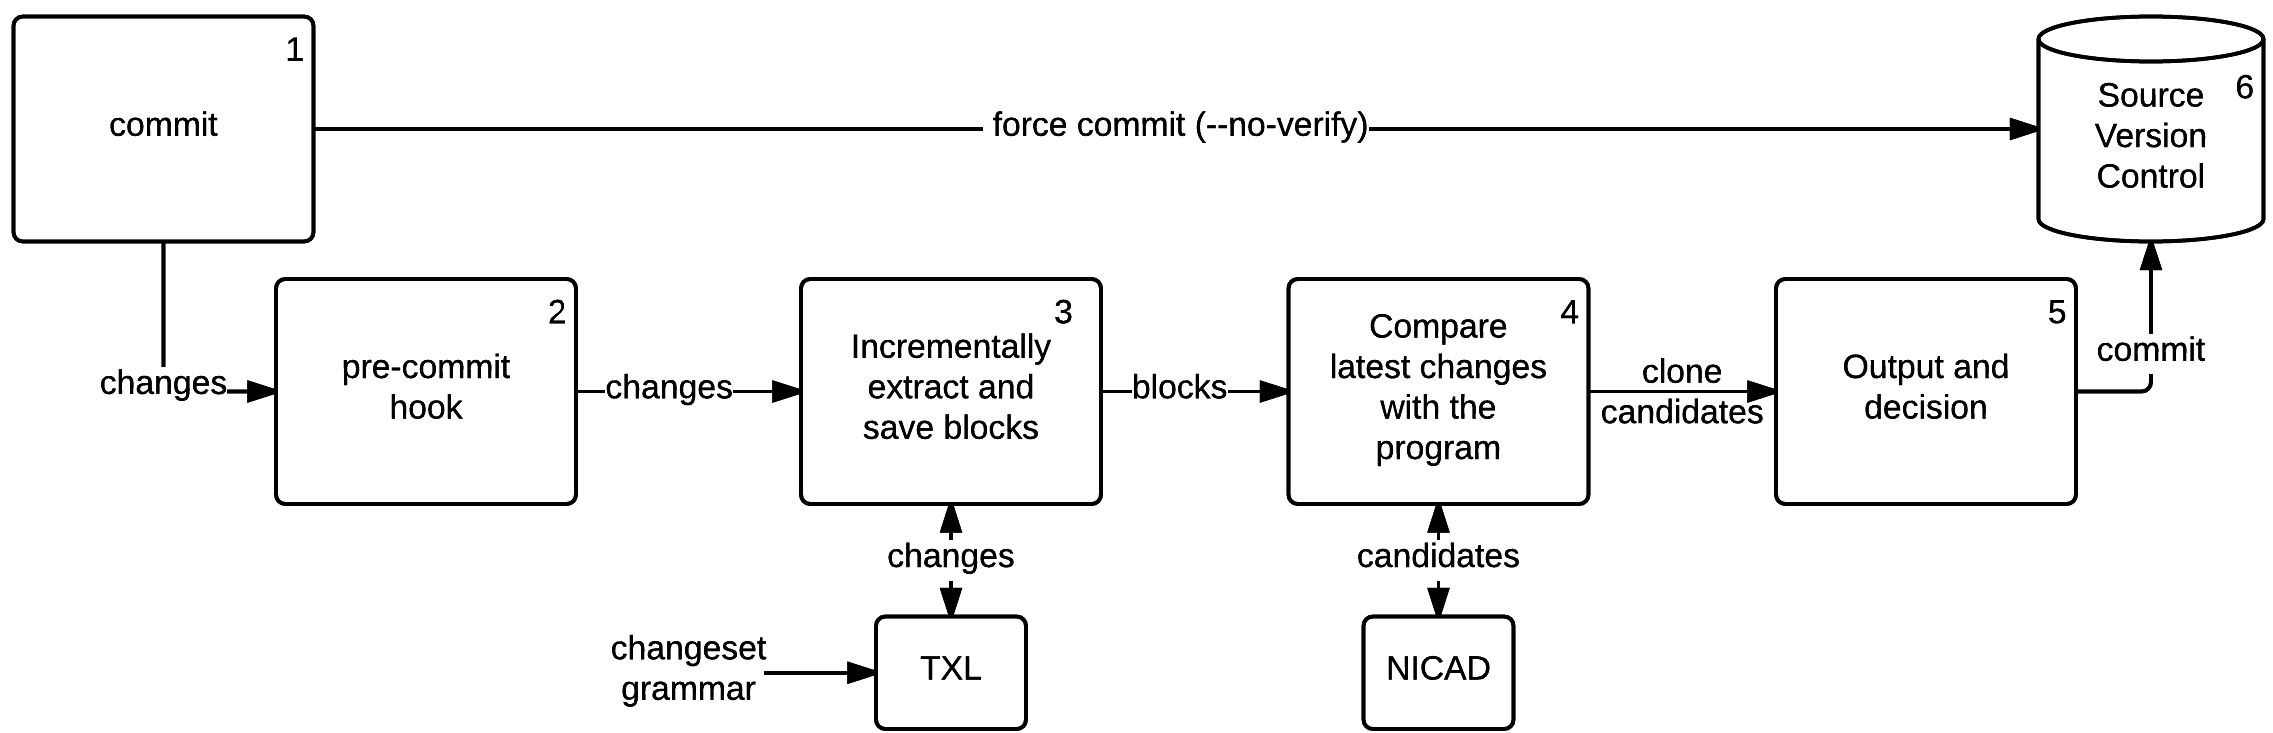
\includegraphics[width=\textwidth]{media/approach.png}
    \caption{ Overview of the PRECINCT Approach.\label{fig:precinct-approach}}
\end{figure*}

The PRECINCT approach is composed of six steps.
The first and last steps are typical steps that a developer would do when committing code.
Indeed, the first step is the commit step where developers send their latest changes to the central repository and the last step is the reception of the commit by the central repository.
The second step is the pre-commit hook, which kicks in as the first operation when one wants to commit.
The pre-commit hook has access to the changes in terms of files that have been modified, more specifically, the lines that have been modified. The modified lines of the files are sent to TXL\cite{Cordy2006a} for block extraction. Then, the blocks are compared to previously extracted blocks in order to identify candidate clones using the comparison engine of NICAD\cite{Cordy2011}. We chose NICAD engine because it has been shown to provide high accuracy \cite{Cordy2011}. The tool is also readily available, easy to use, customizable, and works with TXL. Note, however, that PRECINCT can also work with other engines for comparing code fragments.
Finally, the output of NICAD is further refined and presented to the user for decision.
These steps are discussed in more detail in the following subsections.

\subsubsection{PRECINCT Pre-Commit Hook}
\label{sub:Pre-Commit Hook}

Depending on the exit status of the hook, the commit will be aborted and not pushed to the central repository.
Also, developers can choose to ignore the pre-hook. In Git, for example, they will need to use the command \texttt{git commit --no-verify} instead of \texttt{git commit}.
This can be useful in case of an urgent need for fixing a bug where the code has to reach the central repository as quickly as possible.
Developers can do things like check for code style, check for trailing white spaces (the default hook does exactly this), or check for appropriate documentation on new methods.

PRECINCT is a set of bash scripts where the entry point of these scripts lies in the pre-commit hooks. Pre-commit hooks are easy to create and implement as depicted in Listing~\ref{gitprehook}.
This pre-hook is shipped with Git, a popular version control system.
Note that even though we use Git as the main version control to present PRECINCT, we believe that the techniques presented in this paper are readily applicable to other version control systems.
In Listing~\ref{gitprehook}, from lines 3 to 11, the script identifies if the commit is the first one in order to select the revision to work against.
Then, in Lines 18 and 19, the script checks for trailing whitespace and fails if any are found.

For PRECINCT to work, we just have to add the call to our script suite instead or in addition of the whitespace check.

\noindent\begin{minipage}{0.90\linewidth}

  \lstinputlisting[language=Bash, firstnumber=1, numbers=right, stepnumber=1,leftmargin=30, label=gitprehook, caption=Git Pre-Commit Hook Sample]{media/pre-commit.sample}

\end{minipage}


\subsubsection{Extract and Save Blocks}
\label{sub:Extract and Save Blocks}

A block is a set of consecutive lines of code that will be compared to all other blocks in order to identify clones.
To achieve this critical part of PRECINCT, we rely on TXL\cite{Cordy2006a}, which is a first-order functional programming over linear term rewriting, developed by Cordy et al.\cite{Cordy2006a}.
For TXL to work, one has to write a grammar describing the syntax of the source  language and the transformations needed. TXL has three main phases: \textit{parse, transform}, \textit{unparse}.
In the parse phase, the grammar controls not only the input but also the output form.
Listing~\ref{txlsample} --- extracted from the official documentation\footnote{http://txl.ca} --- shows a grammar matching an \textit{if-then-else} statement in C with some special keywords: [IN] (indent), [EX] (exdent) and [NL] (newline) that will be used for the output form.

\noindent\begin{minipage}{0.90\linewidth}

  \lstinputlisting[language=Bash, firstnumber=1, numbers=right, stepnumber=1,leftmargin=30, label=txlsample, caption=Txl Sample Sample]{media/txl.sample}

\end{minipage}

Then, the \textit{transform} phase will, as the name suggests, apply transformation rules that can, for example, normalize or abstract the source code. Finally, the third phase of TXL,  called \textit{unparse}, unparses the transformed parsed input in order to output it.
Also, TXL supports what the creators call Agile Parsing\cite{Dean}, which allow developers to redefine the rules of the grammar and, therefore, apply different rules than the original ones.


PRECINCT takes advantage of that by redefining the blocks that should be extracted for the purpose of clone comparison, leaving out the  blocks that are out of scope.
More precisely, before each commit, we only extract the blocks belonging to the modified parts of the source code.
Hence, we only process, in an incremental manner, the latest modification of the source code instead of the source code as a whole.

We have selected TXL for several reasons. First, TXL is easy to install and to integrate with the normal workflow of a developer.
Second, it was relatively easy to create a grammar that accepts commits as input.
This is because TXL is shipped with C, Java, Csharp, Python and WSDL grammars that define all the particularities of these languages, with the ability to customize these grammars to accept changesets (chunks of the modified source code that include the added, modified, and deleted lines) instead of the whole code.

\begin{algorithm}
 \KwData{$Changeset[]$ changesets\;
 $Block[]$ prior\_blocks\;
 $Boolean$ compare\_history\;
 }
 \KwResult{Up to date blocks of the systems}
 \For{$i \leftarrow 0$ \KwTo$size\_of~changesets$}{
    Block[] blocks $\leftarrow$ $extract\_blocks(changesets)$\;
    \For{$j \leftarrow 0$ \KwTo$size\_of~blocks$}{
       \If{not $compare\_history$ AND $blocks[j]$ overrides one of $prior\_blocks$}{
          delete $prior\_block$\;
       }
       write $blocks[j]$\;
    }
 }

 \SetKwProg{myproc}{Function}{ $~extract\_blocks(Changeset~cs)$}{}
   \myproc{\proc{}}{

   \uIf{$cs~is~unbalanced~right$}{$cs \leftarrow expand\_left(cs)$\;}

   \ElseIf{$cs~is~unbalanced~left$}{$cs \leftarrow expand\_right(cs)$\;}

   \nl\KwRet$txl\_extract\_blocks(cs)$\;
   }


 \caption{Overview of the Extract Blocks Operation\label{alg:extract}}
\end{algorithm}

\noindent\begin{minipage}{0.90\linewidth}

  \lstinputlisting[language=Bash, firstnumber=1, numbers=right, stepnumber=1,leftmargin=30, label=commitsample, caption=Changeset c4016c of monit]{media/commit.sample}

\end{minipage}


Algorithm~\ref{alg:extract} presents an overview of the ``extract" and ``save" blocks operations of PRECINCT. This algorithm receives as arguments, the changesets, the blocks that have been previously extracted and a boolean named compare\_history.
Then, from Lines 1 to 9 lie the $for$ loop that iterates over the changesets. For each changeset (Line 2), we extract the blocks by calling the $~extract\_blocks(Changeset~cs)$ function.
In this function, we expand our changeset to the left and to the right in order to have a complete block.

As depicted by Listing~\ref{commitsample}, changesets contain only the modified chunk of code and not necessarily complete blocks. Indeed, we have a block from Line 3 to Line 6 and deleted lines from Line 8 to 14.
However, in Line 7 we can see the end of a block, but we do not have its beginning. Therefore, we need to expand the changeset to the left in order to have syntactically correct blocks.
We do so by checking the block's beginning and ending (using \{ and \}) in C for example.
Then, we send these expanded changesets to TXL for block extraction and formalization.

For each extracted block, we check if the current block overrides (replaces) a previous block (Line 4).
In such a case, we delete the previous block as it does not represent the current version of the program anymore (Line 5).
Also, we have an optional step in PRECINCT defined in Line 4. The compare\_history is a condition to delete overridden blocks.

We believe that deleted blocks have been deleted for a good reason (bug, default, removed features, \ldots) and if a newly inserted block matches an old one, it could be worth knowing in order to improve the quality of the system at hand.
This feature is deactivated by default.

In summary, this step receives the files and lines, modified by the latest changes made by the developer and produces an up to date block representation of the system at hand in an incremental way.
The blocks are analysed in the next step to discover potential clones.

\subsubsection{Compare Extracted Blocks}
\label{sub:Compare Extracted Blocks}

In order to compare the extracted blocks and detect potential clones, we can only resort to text-based techniques.
This is because lexical and syntactic analysis approaches (alternatives to text-based comparisons) would require a complete program to work, a program that compiles.
In the relatively wide-range of tools and techniques that exist to detect clones by considering code as text\cite{Johnson1993,Johnson1994,Marcus,Manber1994,StephaneDucasse,Wettel2005}, we selected NICAD as the main text-based method for comparing clones \cite{Cordy2011} for several reasons.
First, NICAD is built on top of TXL, which we also used in the previous step.
Second, NICAD is able to detect all Types 1, 2 and 3 software clones.

NICAD  works in three phases: \textit{Extraction}, \textit{Comparison} and \textit{Reporting}. During the \textit{Extraction} phase all potential clones are identified, pretty-printed, and extracted.
We do not use the \textit{Extraction} phase of NICAD as it has been built to work on programs that are syntactically correct, which is not the case for changesets.
We replaced NICAD's \textit{Extraction} phase with our own scripts, described in the previous section.

In the \textit{Comparison} phase, extracted blocks are transformed, clustered and compared in order to find potential clones.
Using TXL sub-programs, blocks go through a process called pretty-printing where they are stripped of formatting and comments.
When code fragments are cloned, some comments, indentation or spacing are changed according to the new context where the new code is used. This pretty-printing process ensures that all code will have the same spacing and formatting, which renders the comparison of code fragments easier.
Furthermore, in the pretty-printing process, statements can be broken down into several lines.
Table~\ref{tab:pretty-printing} shows how this can improve the accuracy of clone detection with three \texttt{for} statements, \texttt{ for (i=0; i<10; i++)}, \texttt{for (i=1; i<10; i++)} and \texttt{ for (j=2; j<100; j++)}.
The pretty-printing allows NICAD to detect Segments 1 and 2 as a clone pair because only the initialization of $i$ changed.
This specific example would not have been marked as a clone by other  tools we tested such as Duploc\cite{Ducasse1999}.
In addition to the pretty-printing, code can be normalized and filtered to detect different classes of clones and match user preferences.

\begin{table}[]
\centering
\caption{Pretty-Printing Example\cite{Iss2009}}
\label{tab:pretty-printing}
\resizebox{0.5\textwidth}{!}{%
\begin{tabular}{l|l|l|l|l|l}
Segment 1          & Segment 2          & Segment 3           & S1 \& S2 & S1 \& S3 & S2 \& S3 \\ \hline \hline
for (              & for (              & for (               & 1        & 1        & 1        \\
i = 0;             & i = 1;             & j = 2;              & 0        & 0        & 0        \\
i \textgreater 10; & i \textgreater 10; & j \textgreater 100; & 1        & 0        & 0        \\ 
i++)               & i++)               & j++)                & 1        & 0        & 0        \\ \hline \hline
\multicolumn{3}{c|}{Total Matches}                            & 3        & 1        & 1        \\ \hline
\multicolumn{3}{c|}{Total Mismatches}                         & 1        & 3        & 3
\end{tabular}
}
\end{table}


Finally, the extracted, pretty-printed, normalized and filtered blocks are marked as potential clones using a Longest Common Subsequence (LCS) algorithm\cite{Hunt1977}. Then, a percentage of unique statements can be computed and, depending on a given threshold (see Section~\ref{sec:Experimentations}), the blocks are marked as clones.

The last step of NICAD, which acts as our clone comparison engine, is the \textit{reporting}. However, to prevent PRECINCT from outputting a large amount of data (an issue that many clone detection techniques face), we  implemented our own reporting system, which is also well embedded with the workflow of developers. This reporting system is the subject of the next section.

As a summary, this step receives potentially expanded and balanced blocks from the extraction step.
Then, the blocks are pretty-printed, normalized, filtered and fed to an LCS algorithm in order to detect potential clones.
Moreover, the clone detection in PRECINCT is less intensive than NICAD because we only compare the latest changes with the rest of the program instead of comparing all the blocks with each other.

\subsubsection{Output and Decision}
\label{sub:Output and Decision}

In this final step, we report the result of the clone detection at commit time with respect to the latest changes made by the developer. The process is straightforward. Every change made by the developer goes through the previous steps and is checked for the introduction of potential clones. For each file that is suspected to contain a clone, one line is printed to the command line with the following options: (I) Inspect, (D) Disregard, (R) Remove from the commit as shown by Figure \ref{fig:hook}. In comparison to this simple and interactive output, NICAD outputs each and every detail of the detection result such as the total number of potential clones, the total number of lines, the total number of unique line text chars, the total number of unique lines, and so on. We think that so many details might make it hard for developers to react to these results. A problem that was also raised by Johnson et al. \cite{Johnson2013} when examining bug detection tools.
Then the potential clones are stored in XML files that can be viewed using an Internet browser or a text editor.

\begin{figure}
  \centering
    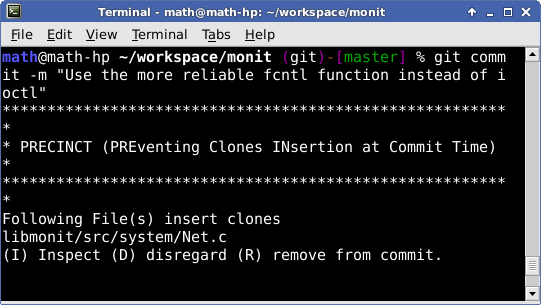
\includegraphics[width=0.48\textwidth]{media/commit.png}
    \caption{PRECINCT output when replaying commit \texttt{710b6b4} of the Monit system used in the case study.\label{fig:hook}}
\end{figure}

(I) Inspect will cause a diff-like visualization of the suspected clones while (D) disregard will simply ignore the finding.
To integrate PRECINCT in the workflow of the developer we also propose the  remove option (R). This option will simply remove the suspected file from the commit that is about to be sent to the central repository.
Also, if the user types an option key twice, e.g., II, DD or RR, then the option will be applied to all files.
For instance, if the developer types DD at any point, the PRECINCT's results will be disregarded and the commit will be allowed to go through. We believe that this simple mechanism will encourage developers to use PRECINCT like they would use any other feature of Git (or any other version control system).


\subsubsection{Case Study}
\label{sec:Experimentations}

In this section, we show the effectiveness of PRECINCT for
detecting clones at commit time in three open source systems\footnote{The programs used and instructions to reproduce the experiments are made available for download from https://research.mathieu-nayrolles.com/precinct/}.

The aim of the case study is to answer the following question: \textit{Can we detect clones at commit time, i.e., before they are inserted in the final code, if so, what would be the accuracy compared to a traditional clone detection tool such as NICAD?}

\subsubsection{Target Systems}
\label{sub:Target Systems}

Table~\ref{tab:sut} shows the systems used in this study and their characteristics in terms of the number files they contain and the size in KLoC (Kilo Lines of Code). We also include the number of revisions used for each system and the programming language in which the system is written.

\begin{table}[]
\centering
\caption{List of Target Systems in Terms of Files and Kilo Line of Code (KLOC) at current version and Language}
\label{tab:sut}
\resizebox{0.5\textwidth}{!}{%
\begin{tabular}{c|c|c|c|c}
SUT        & Revisions & Files & KLoC & Language \\ \hline\hline
Monit      & 826       & 264   & 107  & C        \\ \hline
Jhotdraw   & 735       & 1984  & 44   & Java     \\ \hline
dnsjava    & 1637      & 233   & 47   & Java     \\ \hline
\end{tabular}
}
\end{table}

Monit\footnote{https://mmonit.com/monit/} is a small open source utility for managing and monitoring Unix systems.
Monit is used to conduct automatic maintenance and repair and supports the ability to identify causal actions to detect errors.
This system is written in C and composed of 826 revisions, 264 files, and the latest version has 107 KLoC.
We have chosen Monit as a target system because it was one of the systems NICAD was tested on.

JHotDraw\footnote{http://www.jhotdraw.org/} is a Java GUI framework for technical and structured graphics.
It has been developed as a ``design exercise''. Its design relies heavily on the use of design patterns. JHotDraw is composed of 735 revisions, 1984 files, and the latest revision has 44 KLoC. It is written in Java and it is often used by researchers as a test bench. JHotDraw was also used by NICAD's developers to evaluate their approach.

Dnsjava\footnote{http://www.dnsjava.org/} is a tool for implementing the DNS (Domain Name Service) mechanisms in Java.
This tool can be used for queries, zone transfers, and dynamic updates.
It is not as large as the other two, but it still makes an interesting case subject because it has been well maintained for the past decade. Also, this tool is used in many other popular tools such as Aspirin, Muffin and
Scarab. Dnsjava is composed of 1637 revisions, 233 files, the latest revision contains 47 KLoC.
We have chosen this system because we are familiar with it as we used it before\cite{Nayrolles2015c}.

\subsubsection{Process}
\label{sub:Process}


Figure \ref{fig:precinct-branching} shows the process we followed to validate the effectiveness of PRECINCT.

\begin{figure}
  \centering
    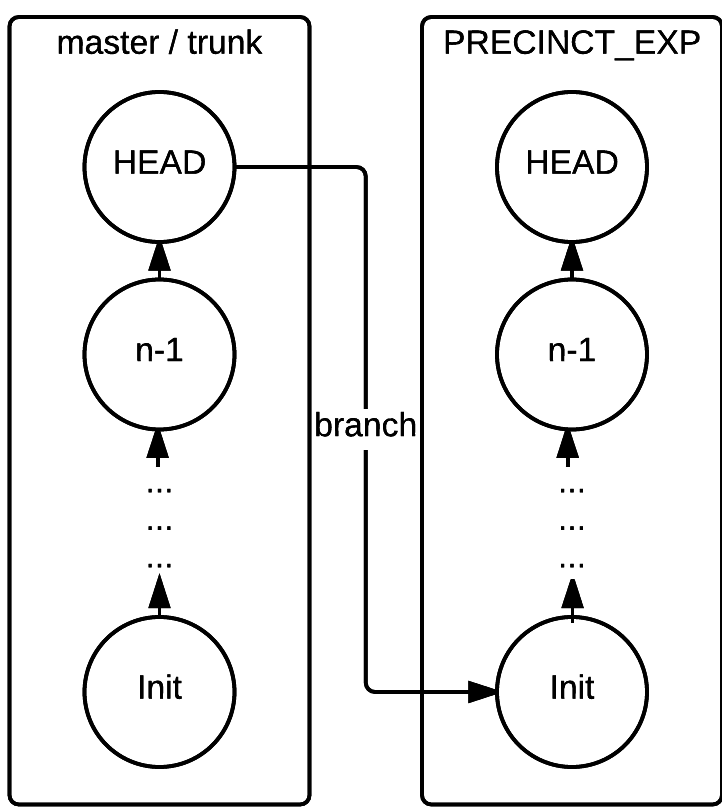
\includegraphics[width=0.3\textwidth]{media/branch.png}
    \caption{PRECINCT Branching.\label{fig:precinct-branching}}
\end{figure}

As our approach relies on commit pre-hooks to detect possible clones during the development process (more particularly at commit time), we had to find a way to \textit{replay} past commits. To do so, we  \textit{cloned} our test subjects, and then created a new branch called \textit{PRECINCT\_EXT}.
When created, this branch is reinitialized at the initial state of the project (the first commit) and each commit can be replayed as they have originally been. At each commit, we store the time taken for PRECINCT to run as well as the number of detected clone pairs. We also compute the size of the output in terms of the number of lines of text output by our method. The aim is to reduce the output size to help software developers interpret the results.

To validate the results obtained by PRECINCT, we needed to use a reliable clone detection approach to extract clones from the target systems and use these clones as a baseline for comparison. For this, we turned to NICAD because of its popularity, high accuracy, and availability \cite{Cordy2011}, as discussed before. This means, we run NICAD on the revisions of the system to obtain the clones then we used NICAD clones as a baseline for comparing the results obtained by PRECINCT.

It may appear strange that we are using NICAD to validate our approach, knowing that our approach uses NICAD's code comparison engine. In fact, what we are assessing here is the ability for PRECINCT to detect clones at commit time using changsets. The major part of PRECINCT is the ability to  intercept code changes and build working code blocks that are fed to a code fragment engine (in our case NICAD's engine). PRECINCT can be built on the top of any other code comparison engine.

We show the result of detecting Type 3 clones with a maximum line difference of 30\% as discussed in Table~\ref{tab:result}. As discussed in the introductory section, we chose to report on Type 3 clones because they are more challenging to detect than Type 1 and 2. PRECINCT detects Type 1 and 2 too so does NICAD. For the time being, PRECINCT is not designed to detect Type 4 clones. These clones use different implementations. Detecting Type 4 clones is part of future work.

% [WAHAB: YOU NEED TO DEFINE PRECISION AND RECALL]

We assess the performance of PRECINCT in terms of precision (Equation 1) and recall (Equation 2).
Both precision and recall are computed by considering  NICAD's results as a baseline.
We also compute F$_{1}$-measure (Equation 3), i.e., the weighted average of precision and recall, to measure the accuracy of PRECINCT.

\begin{equation}
precision = \frac{|\{ NICAD_{detection} \} \cap \{ PRECINCT_{detection} \} |}{| \{ PRECINCT_{detection} \}|}
\end{equation}

\begin{equation}
recall = \frac{|\{ NICAD_{detection} \} \cap \{ PRECINCT_{detection} \} |}{| \{ NICAD_{detection} \}|}
\end{equation}

\begin{equation}
F_1-measure = 2 * \frac{precision * recall}{precision + recall}
\end{equation}


\begin {figure*}%[!hbtp]
\centering
\begin{tikzpicture}
    \begin{axis}[
      scale only axis, % The height and width argument only apply to the actual axis
    height=5cm,
    width=0.9\textwidth,
    grid = both,
    minor tick num=1,
    xlabel={Revisions},
    ylabel={Clones},
    xmin=0]
    \addplot table [smooth,red,mark=none,x=revision,y=clones,col sep=comma] {methodology/data/monit};
    \addlegendentry{NICAD Detection}

    \addplot table [smooth,blue,mark=none,x=revision,y=detected,col sep=comma] {methodology/data/monit};
    \addlegendentry{PRECINCT Detection}

    \addplot table [smooth,red,mark=none,x=revision,y=prevented,col sep=comma] {methodology/data/monit};
    \addlegendentry{Remaining Clones}

    \end{axis}
    \end{tikzpicture}
    \caption{Monit clone detection over revisions\label{fig:r1}}
\end{figure*}

\begin {figure*}%[!hbtp]
\centering
\begin{tikzpicture}
    \begin{axis}[
      scale only axis, % The height and width argument only apply to the actual axis
    height=5cm,
    width=0.9\textwidth,
    grid = both,
    minor tick num=1,
    xlabel={Revisions},
    ylabel={Clones},
    xmin=0]
  \addplot table [smooth,red,mark=none,x=revision,y=clones,col sep=comma] {methodology/data/jhotdraw};
      \addlegendentry{NICAD Detection}

    \addplot table [smooth,green,mark=none,x=revision,y=detected,col sep=comma] {methodology/data/jhotdraw};
    \addlegendentry{PRECINCT Detection}

    \addplot table [smooth,red,mark=none,x=revision,y=prevented,col sep=comma] {methodology/data/jhotdraw};
    \addlegendentry{Remaining Clones}

    \end{axis}
    \end{tikzpicture}
    \caption{JHotDraw clone detection over revisions\label{fig:r2}}
\end{figure*}

\begin {figure*}%[!hbtp]
\centering
\begin{tikzpicture}
    \begin{axis}[
      scale only axis, % The height and width argument only apply to the actual axis
    height=5cm,
    width=0.9\textwidth,
    grid = both,
    minor tick num=1,
    xlabel={Revisions},
    ylabel={Clones},
    xmin=0]
  \addplot table [smooth,red,mark=none,x=revision,y=clones,col sep=comma] {methodology/data/dnsjava};
    \addlegendentry{NICAD Detection}

    \addplot table [smooth,green,mark=none,x=revision,y=detected,col sep=comma] {methodology/data/dnsjava};
    \addlegendentry{PRECINCT Detection}

    \addplot table [smooth,red,mark=none,x=revision,y=prevented,col sep=comma] {methodology/data/dnsjava};
    \addlegendentry{Remaining Clones}

    \end{axis}
    \end{tikzpicture}
    \caption{Dnsjava clone detection over revisions\label{fig:r3}}
\end{figure*}


\subsubsection{Results}
\label{sub:Results}

Figures~\ref{fig:r1},~\ref{fig:r2},~\ref{fig:r3} show the results of our study in terms of clone pairs that are detected per revision for our three subject systems: Monit, JHotDraw and Dnsjava. We used as baseline for comparison the clone pairs detected by NICAD. The blue line shows the clone detection performed by NICAD. The red line shows the clone pairs detected by PRECINCT. The brown line shows the clone pairs that have been missed by PRECINCT. As we can quickly see, the blue and red lines almost overlap, which indicates a good accuracy of the PRECINCT approach.

\begin{table*}[]
\centering
\caption{Overview of PRECINCT's results in terms of precision, recall, F$_{1}$-measure, execution time and output reduction.}
\label{tab:result}

\begin{tabular}{c|c|c|c|c|c||c|c|c}
         & NICAD
         & PREC.
         & Prec.
         & Recall
         & F1
         & \begin{tabular}[c]{@{}c@{}}NICAD'\\  Time\end{tabular}
         & \begin{tabular}[c]{@{}c@{}}PREC.'s\\  Time\end{tabular}
         & \begin{tabular}[c]{@{}c@{}}Output \\  Reduc.\end{tabular} \\ \hline\hline
Monit    & 128   & 123      & 96.1\%    & 100\%  & 98\%       & 2.2s                                                                     & 0.9s                                                                         & 88.3\%                                                              \\ \hline
JHotDraw & 6599  & 6490     & 98.3\%    & 100\%  & 99.1\%     & 5.1s                                                                     & 1.7s                                                                         & 70.1\%                                                              \\ \hline
DnsJava  & 273   & 226      & 82.8\%    & 100\%  & 90.6\%     & 1.8s                                                                     & 1.1s                                                                         & 88.6\%                                                              \\ \hline\hline
Total    & 7000  & 6839     & 97.7\%    & 100\%  & 98.8\%     & 3s                                                                       & 1.2s                                                                         & 83.4\%                                                              \\ \hline
\end{tabular}

\end{table*}


Table~\ref{tab:result} summarizes PRECINCT's results in terms of precision, recall, F$_{1}$-measure, execution time and output reduction.
The first version of Monit contains 85 clone pairs and this number stays stable until Revision 100. From Revision 100 to 472 the detected clone pairs vary between 68 and 88 before reaching 219 at Revision 473.
The number of clone pairs goes down to 122 at Revision 491 and decreases to 128 in the last revision. PRECINCT was able to detect 96.1\% (123/128) of the clone pairs that are detected by NICAD with a 100\% recall.
It took in average around 1 second for PRECINCT to execute on a Debian 8 system with Intel(R) Core(TM) i5-2400 CPU @ 3.10GHz, 8Gb of DDR3 memory.
It is also worth mentioning that the computer we used is equipped with SSD (Solid State Drive).
This impacts the running time as clone detection is a file intensive operation.
Finally, the PRECINCT was able to output 88.3\% less lines than NICAD.

JHotDraw starts with 196 clone pairs at Revision 1 and reaches a pick of 2048 at Revision 180. The number of clones  continues to go up until Revisions 685 and 686 where the number of pairs is 1229 before picking at 6538 and more from Revisions 687 to 721.
PRECINCT was able to detect 98.3\% of the clone pairs detected by NICAD (6490/6599) with 100\% recall while executing on average in 1.7 second (compared to 5.1 seconds for NICAD).
With JHotDraw, we can clearly see the advantages of incremental approaches.
Indeed, the execution time of PRECINCT is loosely impacted by the number of files inside the system as the blocks are constructed incrementally.
Also, we only compare the latest change to the remaining of the program and not all the blocks to each other as NICAD.
We also were able to reduce by 70.1\% the number of lines output by NICAD.

Finally, for Dnsjava, the number of clone pairs starts high with 258 clones and goes up until Revision 70 where it reaches 165. Another quick drop is observed at Revision 239 where we found only 25 clone pairs. The number of clone pairs stays stable until Revision 1030 where it reaches 273. PRECINCT was able to detect 82.8\% of the clone pairs detected by NICAD (226/273) with 100\% recall, while executing on average in 1.1 second while NICAD took 3 seconds in average. PRECINCT outputs  83.4\% less lines of code than NICAD.

Overall, PRECINCT prevented 97.7\% of the 7000 clones (in all systems) to reach the central source code repository while executing more than twice as fast as NICAD (1.2 seconds compared to 3 seconds in average) while reducing the output in terms of lines of text output the developers by 83.4\% in average. Note here that we have not evaluated the quality of the output of PRECINCT compared to NICAD's output. We need to conduct user studies for this. We are, however, confident, based on our own experience trying many clone detection tools, that a simpler and more interactive way to present the results of a clone detection tool is warranted. PRECINCT aims to do just that.

The difference in execution time between NICAD and PRECINCT stems from the fact that, unlike PRICINCT, NICAD is not an incremental approach. For each revision, NICAD has to extract all the code blocks and then compares all the pairs with each other. On the other hand, PRECINCT only extracts blocks when they are modified and only compares what has been modified with the rest of the program.

The difference in precision between NICAD and PRECINCT (2.3\%)  can be explained by the fact that sometimes developers commit code that does not compile.
Such commits will still count as a revision, but TXL fails to extract blocks that do not comply with the target language syntax.
While NICAD also fails in such a case, the disadvantage of PRECINCT comes from the fact that the failed block is saved and used as reference until it is changed by a correct one in another commit.

\subsubsection{Threats to Validity}
\label{sec:Threats to Validity}

The selection of target systems is one of the common threats to validity for approaches aiming to improve the analysis of software systems.
It is possible that the selected programs share common properties that we are not aware of and therefore, invalidate our results.
However, the systems analysed by PRECINCT are the same as the ones used in similar studies.
Moreover, the systems  vary in terms of purpose, size and history.

In addition, we see a threat to validity that stems from the fact that we only used open source systems. The results may not be generalizable to industrial systems. We intend to undertake these studies in future work.

The programs we used in this study are all based on the Java, C and Python programming languages. This can limit the generalization of the results. However, similar to Java, C, Python, if one writes a TXL grammar for a new language --- which can be a relatively hard work --- then PRECINCT can work since PRECINT relies on TXL.

Finally, we use NICAD as the code comparison engine. The accuracy of NICAD affects the accuracy of PRECINCT. This said, since NICAD has been tested on large systems, we are confident that it is a suitable engine for comparing code using TXL. Also, there is nothing that prevents us from using other code comparisons engines, if need be.

In conclusion, internal and external validity have both been minimized by choosing a set of three different systems, using input data that can be found in any programming languages and version systems (commit and changesets).


\subsubsection{Conclusion}
\label{sec:Conclusion}

PRECINCT (PREventing Clones INsertion at Commit Time) iq an incremental approach for preventing clone insertion at commit time that combines efficient block extraction and clone detection and integrate itself seamlessly in the day-to-day workflow of developers.
PRECINCT takes advantage of TXL and NICAD to create a clone detection tool approach that runs automatically before each commit in 1.2 second with a 97.7\% precision and a 100\% recall (when using NICAD results as a baseline).

Our approach also assesses two major factors that contribute to the slow adoption of clone detection tools: large number of data output by clone detection methods,  and  smooth integration with the task flow of the developers.
PRECINCT is able to reduce the number of lines output by a classical clone detection tool such as NICAD by 83.4\% while keeping all the necessary information that allow developers to decide whether the detect clone is in fact a clone.
Also, our approach is seamlessly integrated with the developers' workflow by means of pre-commit hooks, which are part any version control systems.

To build on this work, we need to experiment with additional (and larger) systems with the dual aim to (a) improve and fine-tune the approach, and (b) assess the scalability of our approach when applied to even larger (and proprietary) systems. Also, we want to improve PRECINCT to support Type 4 clones.



\chapter{Preventing Bug Insertion Using Clone Detection\label{chap:bianca}}

%!TEX root = ../research_proposal.tex


{\tt BIANCA} (Bug Insertion ANticipation by Clone Analysis at merge time) is the final piece of the proposed ecosystem and, as such, the final failsafe that prevents developer to ship code that we know to be sub-optimum or to be at the very root of issues.

Many tools exist to prevent a developer to ship {\it bad} code \cite{Dangel2000,Hovemeyer2007,Moha2010} or to identify {\it bad} code after executions (e.g in test or production environment) \cite{Nayrolles,Nayrolles2013a}.
However, these tools rely on metrics and rules to statically and/or dynamically identify sub-optimum code.

\subsubsection{The {\tt BIANCA} approach\label{sec:bianca-approach}}

{\tt BIANCA} is different than the approaches presented in the previous sections  because it mines and analyzes the change patterns in commits and matches it against past commits known to have introduced a defect in the code (or that have just been replaced by better implementation).
Also, {\tt BIANCA} is an offline approach that is triggered by a merge request.
When a maitainers estimate that their work are ready to be integrated with the main branch, they open a merge request\footnote{Also known as pull request}.
Merging a task branch is not an instanteous process as the code need to pass code review.
{\tt BIANCA} leverages this {\it down} time to perform a complete history check on all projects contained in {\tt BUMPER}.

Figure \ref{fig:bianca-approach} presents an overview of our approach.

\begin{figure}[h!]
  \centering
    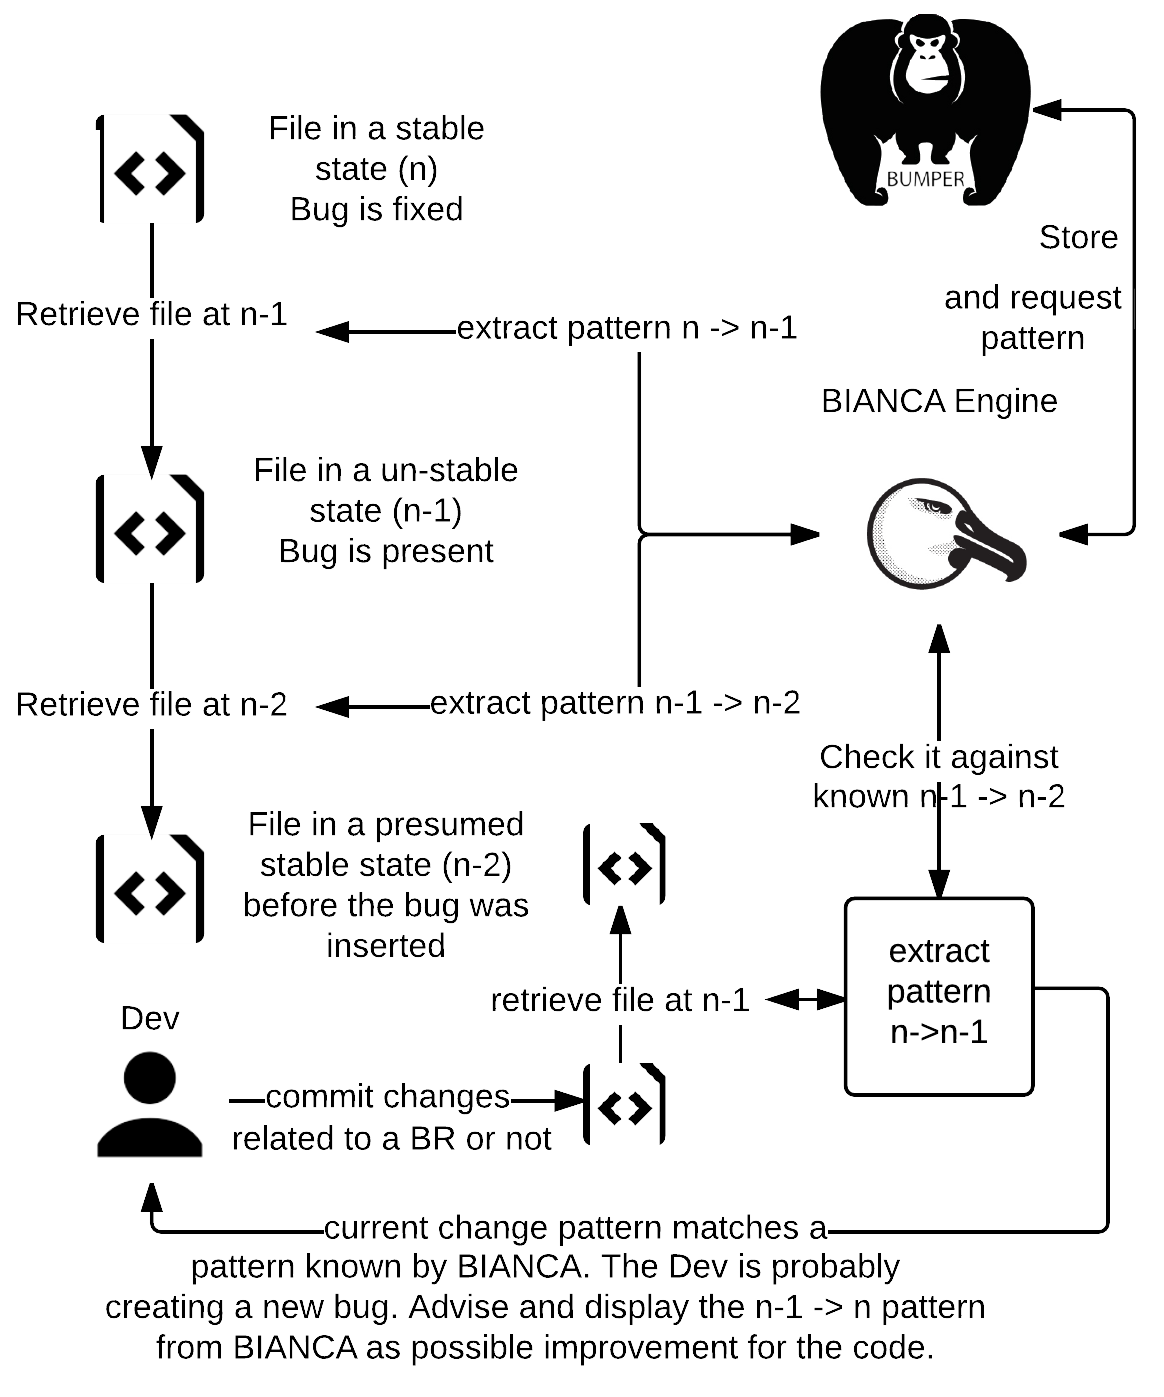
\includegraphics{media/bianca-approach.png}
    \caption{The BIANCA Approach
    \label{fig:bianca-approach}}
\end{figure}

{\tt BIANCA} builds a model where each issue is represented by three versions of the same file.
These three versions are stored in {\tt BUMPER}.
The first version $n$ is called the {\it stable state} because the code of this version was used to fix an issue.
The $n-1$ version, however, is called the {\it unstable state} as it was marked as containing an issue.
Finally, the third version is called the {\it before state} and represents the file before the introduction of the bug.
Hereafter, we refer to the {\it before state} as $n-2$.
{\tt BIANCA} extracts the change patterns form $n-2$ to $n-1$ and from $n-1$ to $n$.
It aslo generates the changes to go from $n-2$ to $n$.

When a developer commits new modifications, {\tt BIANCA} extracts the change pattern from the version $n_{dev}$ (current version) and $n-1_{dev}$ (version before modification) of the developer's source code and compare this change patterns to known $n-2$ to $n-1$ patterns.
If $n_{dev}$ to $n-1_{dev}$ matches a $n-2$ to $n-1$ then it means that the developer is inserting a known defect in the source code.
In such a case, {\tt BIANCA} will propose the related $n-1$ to $n$ pattern to the developer, so s/he could improve the source code and will show the related $n-2$ for the $n$ pattern so the developer will learn how to s/he should have modified the code in the first place.

Moreover, if the issue was previously reproduced by {\tt JCHARMING}, then {\tt BIANCA} will display the step to reproduce it.


To extract the change patterns and compare them, we used the same technique as the one presented in section \ref{sub:Extract and Save Blocks}.
The third and the fourth normalizations are removing all {\it less} important calls in the normalization one and two of {\tt RESEMBLE}.
We classify a call as less-important if, for example, it only does display-related functionalities such as generating HTML or printing something to the console. Finally, the fourth normalization will transform the code to an intermediate language of our own that will allow us to compare source code implemented in different programming languages.

Then, as in {\tt RESEMBLE}, if the LCS is above a user-defined threshold, then a warning is raised by {\tt BIANCA} alerting the developer that the commit is suspected to insert a defect.
The given defect is shown to the developer and can either force the commit if s/he don't find the warning relevant or abort the commit.

We believe that the warning, alongside the previously mined change patterns and steps to reproduce the suspected default --- provided by {\tt JCHARMING}, if available --- will statisfy developers in terms of actionable inteligence.
Thus, {\tt BIANCA} could succeed, where other tools failed, at being used in industrial environment	\cite{Lewis2013}.


\subsubsection{Early experiments}

We have experimented the efficiency of {\tt BIANCA} with the same datasets we used to build our bug taxonomy proposed in section \ref{chap:taxonomy}.

\begin{table}[h]
\begin{center}
\begin{tabular}{@{}c|c|c|c|c@{}}
\textbf{Dataset} & \textbf{Fixed Issues} & \textbf{Commit} & \textbf{Files} & \textbf{Projects} \\ \hline \hline
Netbeans         & 53,258          & 122,632     & 30,595         & 39                \\
Apache           & 49,449          & 106,366     & 38,111         & 349               \\
Total            & 102,707         & 229,153     & 68,809         & 388               \\ \hline \hline

\end{tabular}
\end{center}

\caption{Datasets\label{table:datasets-bianca}}
\end{table}

We choosed to use the same datasets for several reasons. First of all, we spare the time needed to collect new datasets. Then, because these datasets contain a very large system mainly implemented in Java: Netbeans; and 349 independent Apache projects implemented in a very wide range of programming language. Consequently, these datasets allow us to test the efficiency of our different code normalizations.

We ran two different experiments using the two first normalizations we described in section \ref{sec:bianca-approach}. Both experiments consider only a few months of history, from April to August 2008. While this could hinder the pertinence of our results, these five months of history contain 167,597 commits related to bug fix. Consequently, we believe our results to be representative.

The first experiment yields the result presented by Figure \ref{fig:bianca-exp-1}.

\begin{figure}[h!]
  \centering
    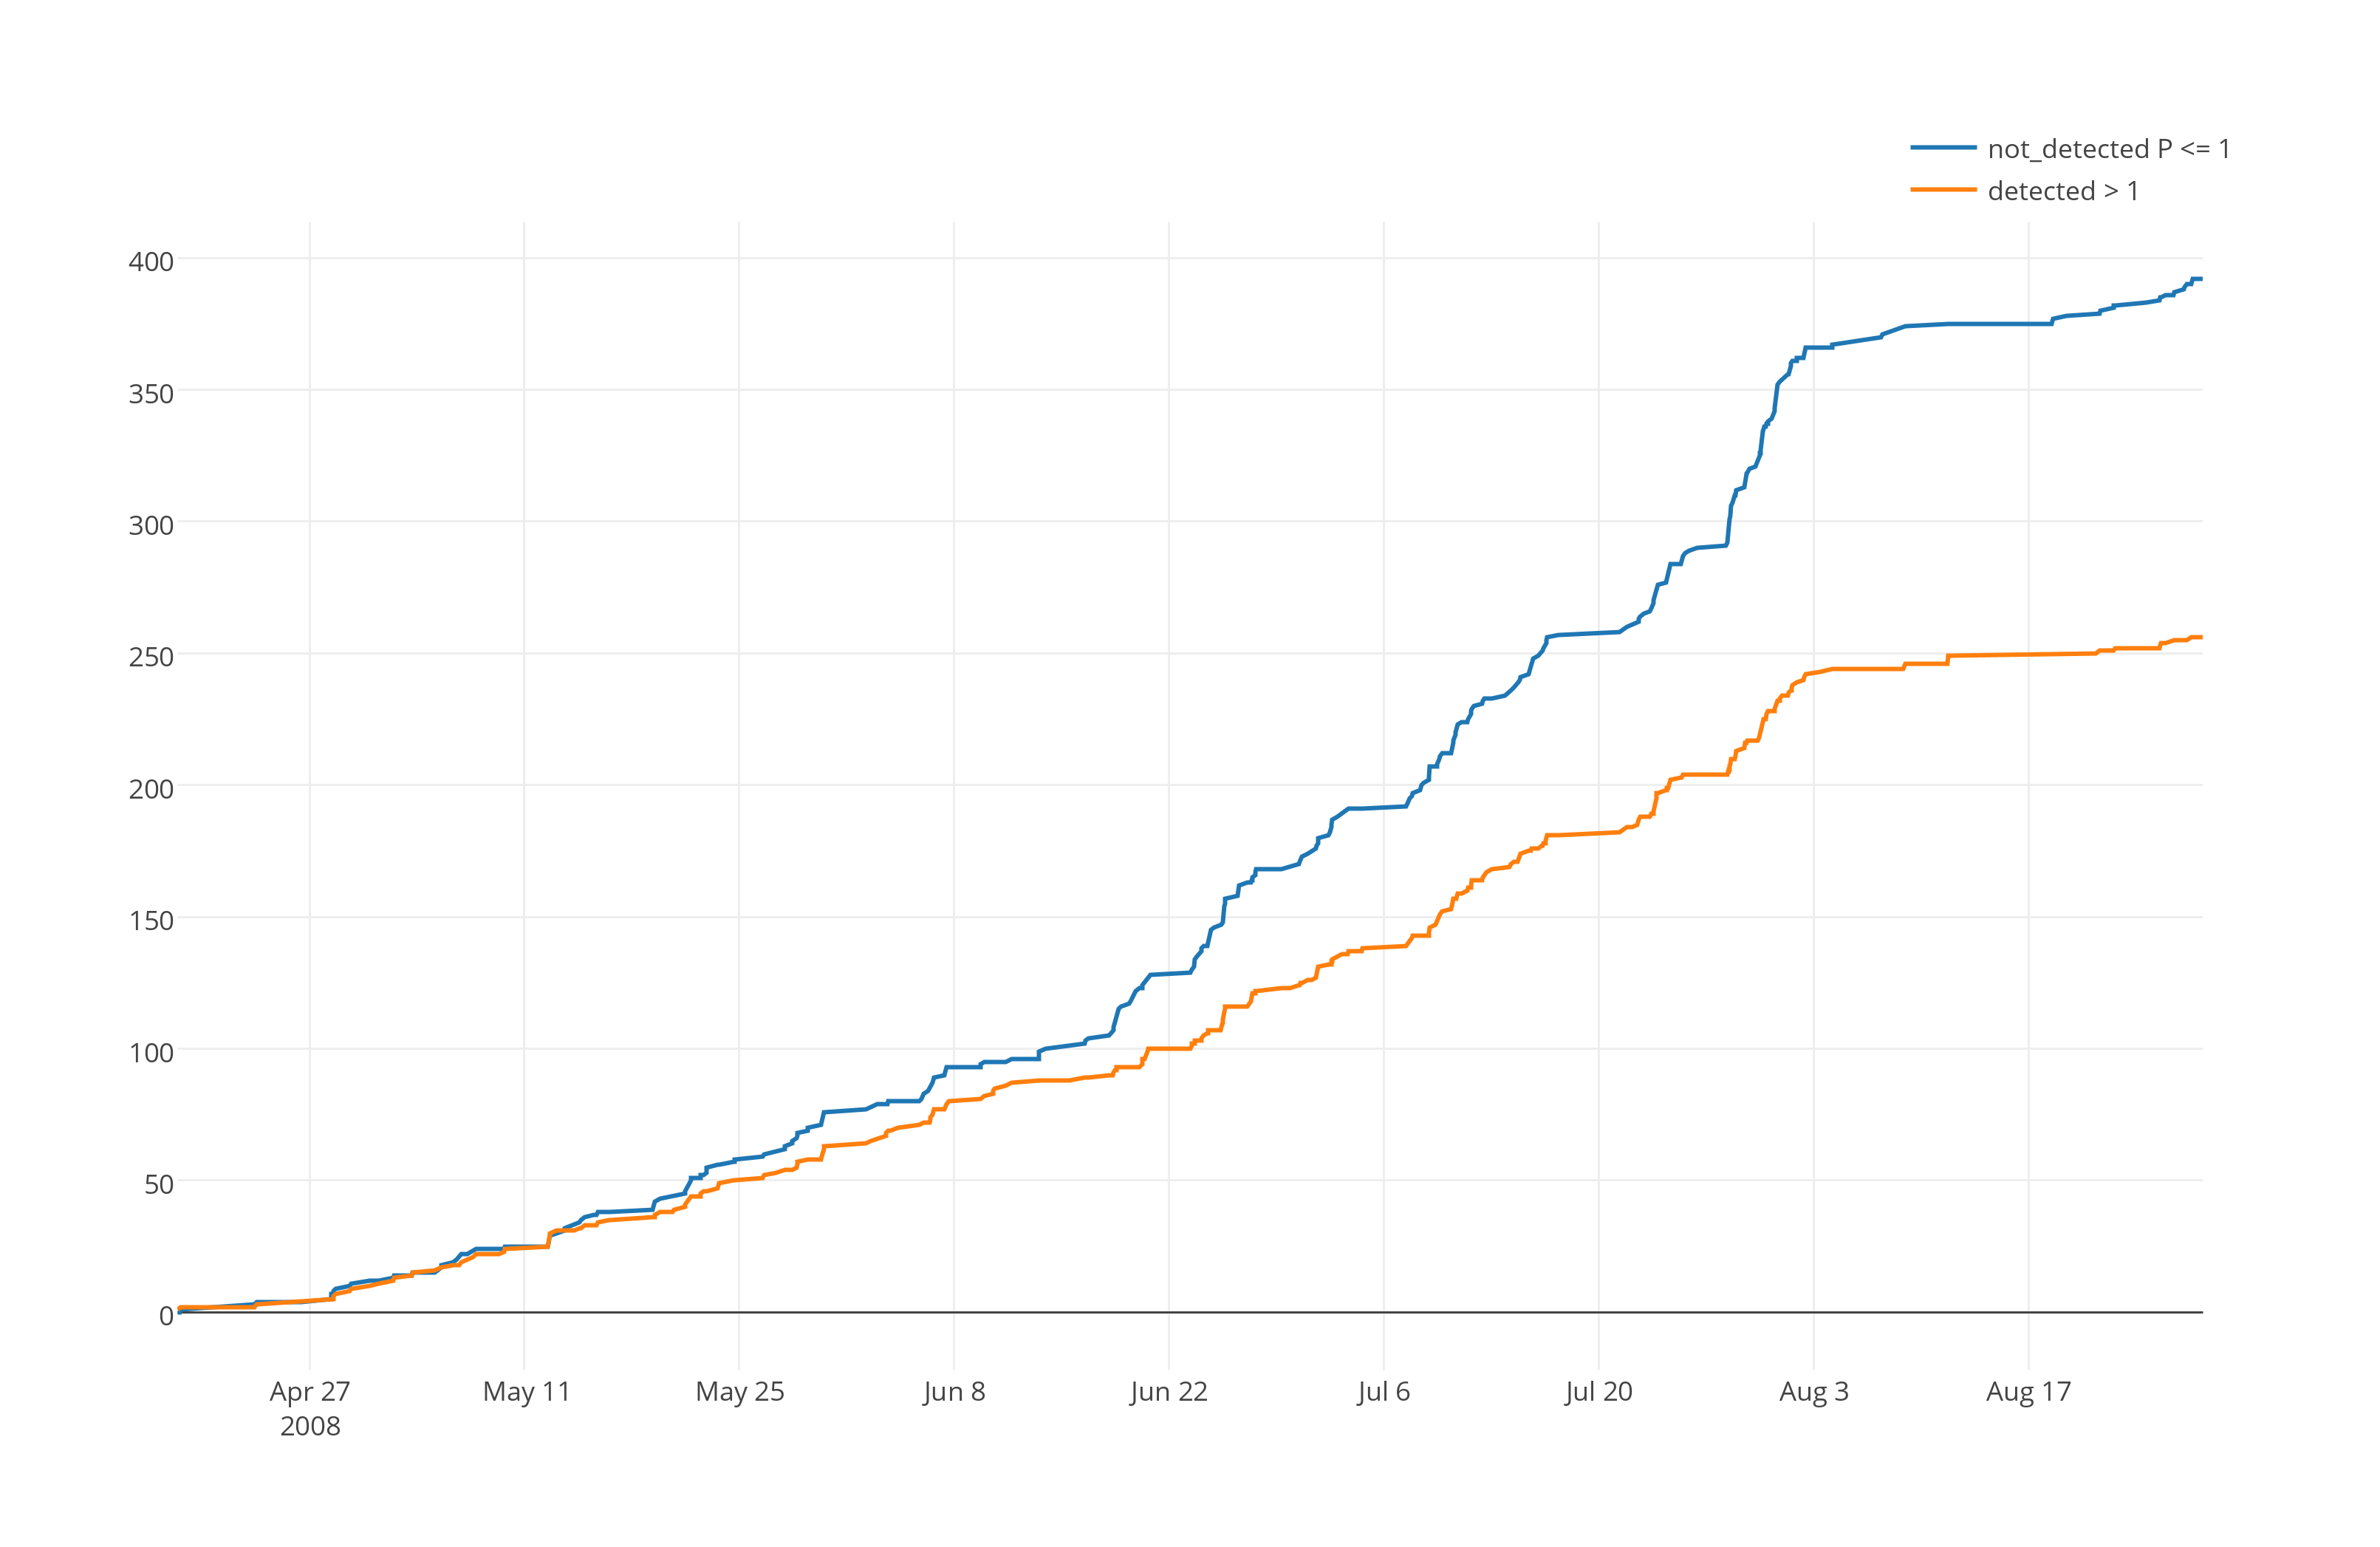
\includegraphics[scale=0.55]{media/bianca-13.png}
    \caption{{\tt BIANCA} warnings from April to August 2008 using the first normalization.
    \label{fig:bianca-exp-1}}
\end{figure}

With the first normalization, {\tt BIANCA} raised 69,519 warnings out of 167,597 (41.5\%) analyzed commits.
Out of these 69,519, 13.4\% turned out to be false positives. A false positive is a commit that have been tagged as introducing a bug by {\tt BIANCA} but did not according to the history.
However, false positives have to be dealt with carefully in this study as the commit might have introduced a bug but the bug could have not been reported yet.

In our second experiment, we used the second normalization and {\tt BIANCA} raised 83,627 warnings out of 167,597 (48.89\%) commit we analyze. However, the false positive rate increases to 21\%. Figure \ref{fig:bianca-exp-2} shows the results.

\begin{figure}[h!]
  \centering
    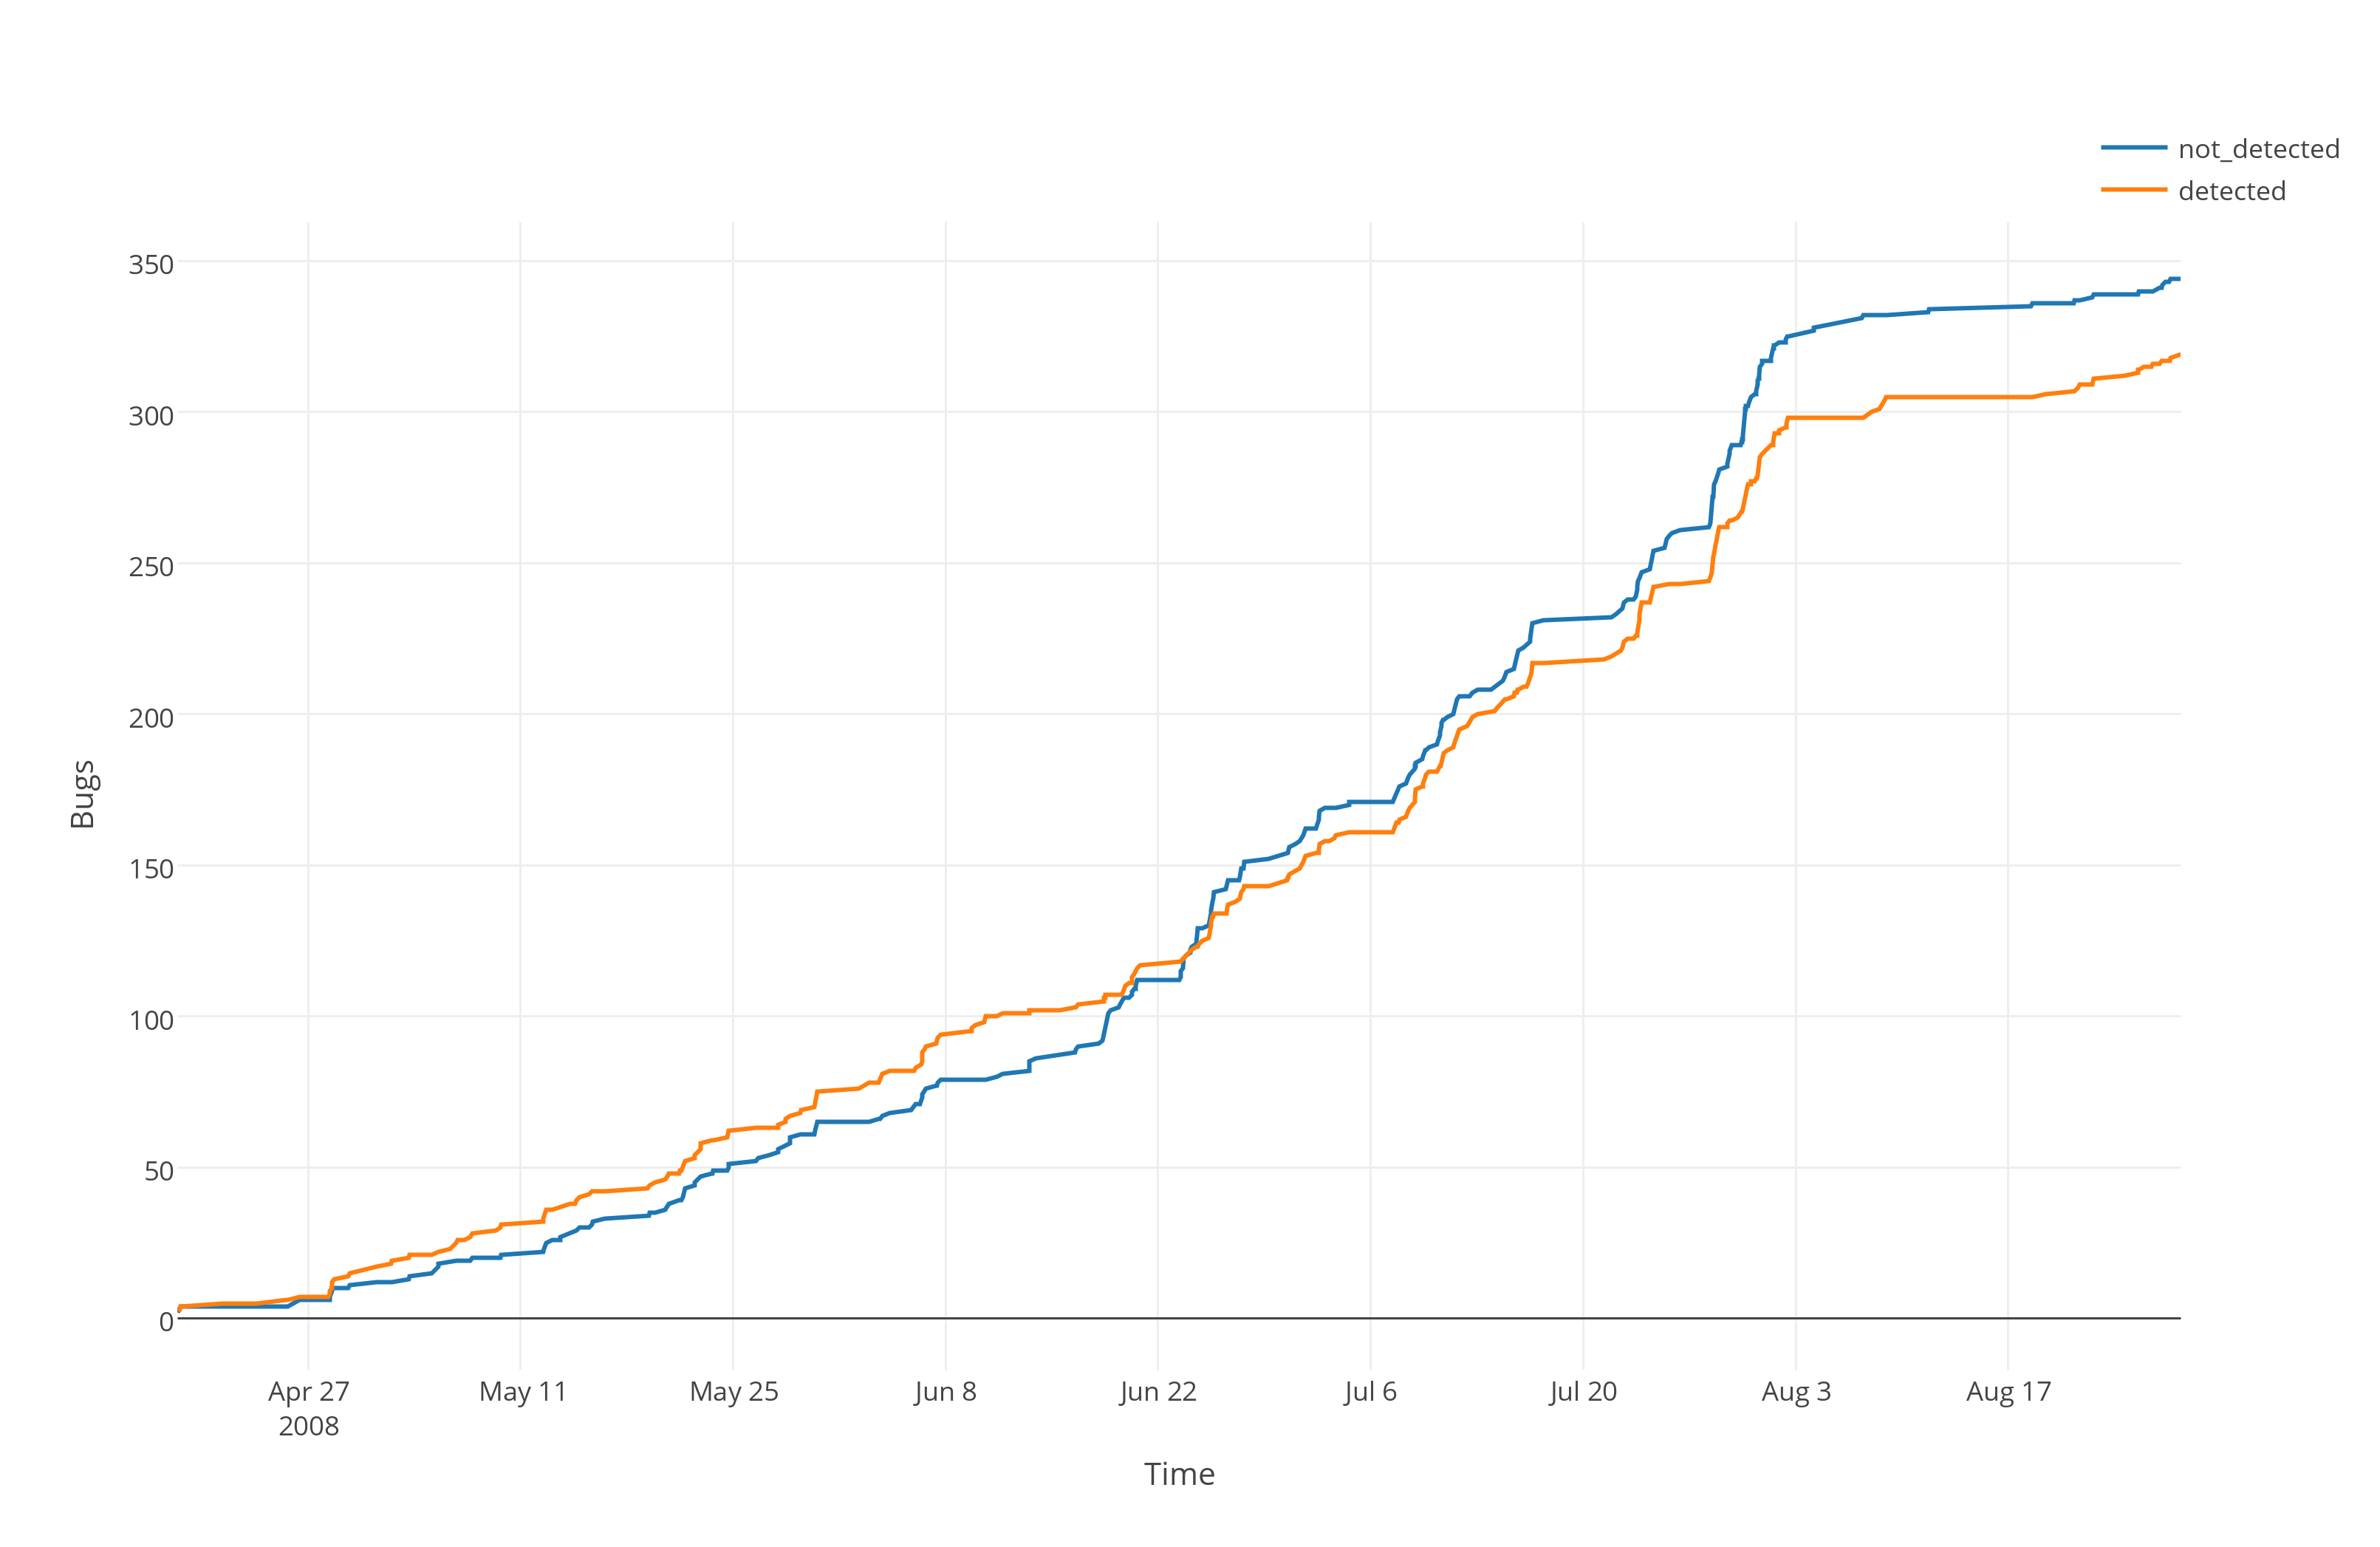
\includegraphics[scale=0.55]{media/bianca-20.png}
    \caption{{\tt BIANCA} warnings from April to August 2008 using the second normalization.
    \label{fig:bianca-exp-2}}
\end{figure}

{\tt BIANCA} experiments are still in their early stage and we are still trying to improve our normalizations in order to reduce the false positive rate.


% \chapter{A Bug Classification Approach Based on the Locations of the Corrections --- An Empirical Study\label{chap:taxonomy}}
%
% %!TEX root = ../research_proposal.tex

In order to classify the research on the different fields related to software maintenance, we can reason about types of bugs at different levels. For
example, we can group bugs based on the developers that fix
them or using information about the bugs such as crash traces.


Our aim is not to improve testing as it is the case in the work of Eldh \cite{Eldh2001} and Hamill et al.\cite{Hamill2014}.
Our objective is to propose a classification that can allow researchers in the filed of mining bug 9 repositiories to use the taxonomy as a new criterion in triaging, prediction, and reproduction of bugs.
By analogy, we can look at the proposed bug taxonomy in a similar way as the clone taxonomy presented by Kapser and Godfrey \cite{CoryKapser}.
The authors proposed seven types of source code clones and then conducted a case study, using their classification, on the file system module of the Linux operating system.
This clone taxonomy continues to be used by researchers to build better approaches for detecting a given clone type and being able to effectively compare approaches with each other.

In this section, we are interested in bugs that share similar fixes.
By a fix, we mean a modification (adding or deleting lines of
code) to an exiting file that is used to solve the bug. With this
in mind, the relationship between bugs and fixes can be
modeled using the UML diagram in Figure \ref{fig:bug-taxo-diag}. The diagram
only includes bugs that are fixed. From this figure, we can
think of four instances of this diagram, which we refer to as
bug taxonomy or simply bug types (see Figure \ref{fig:bug-taxo}).



\begin{figure}[h!]
  \centering
    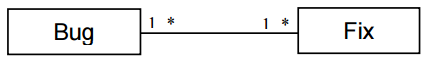
\includegraphics[scale=0.5]{media/bug-taxo-class-diag.png}
    \caption{Class diagram showing the relationship between bugs and fixed
    \label{fig:bug-taxo-diag}}
\end{figure}

\begin{figure}[h!]
  \centering
    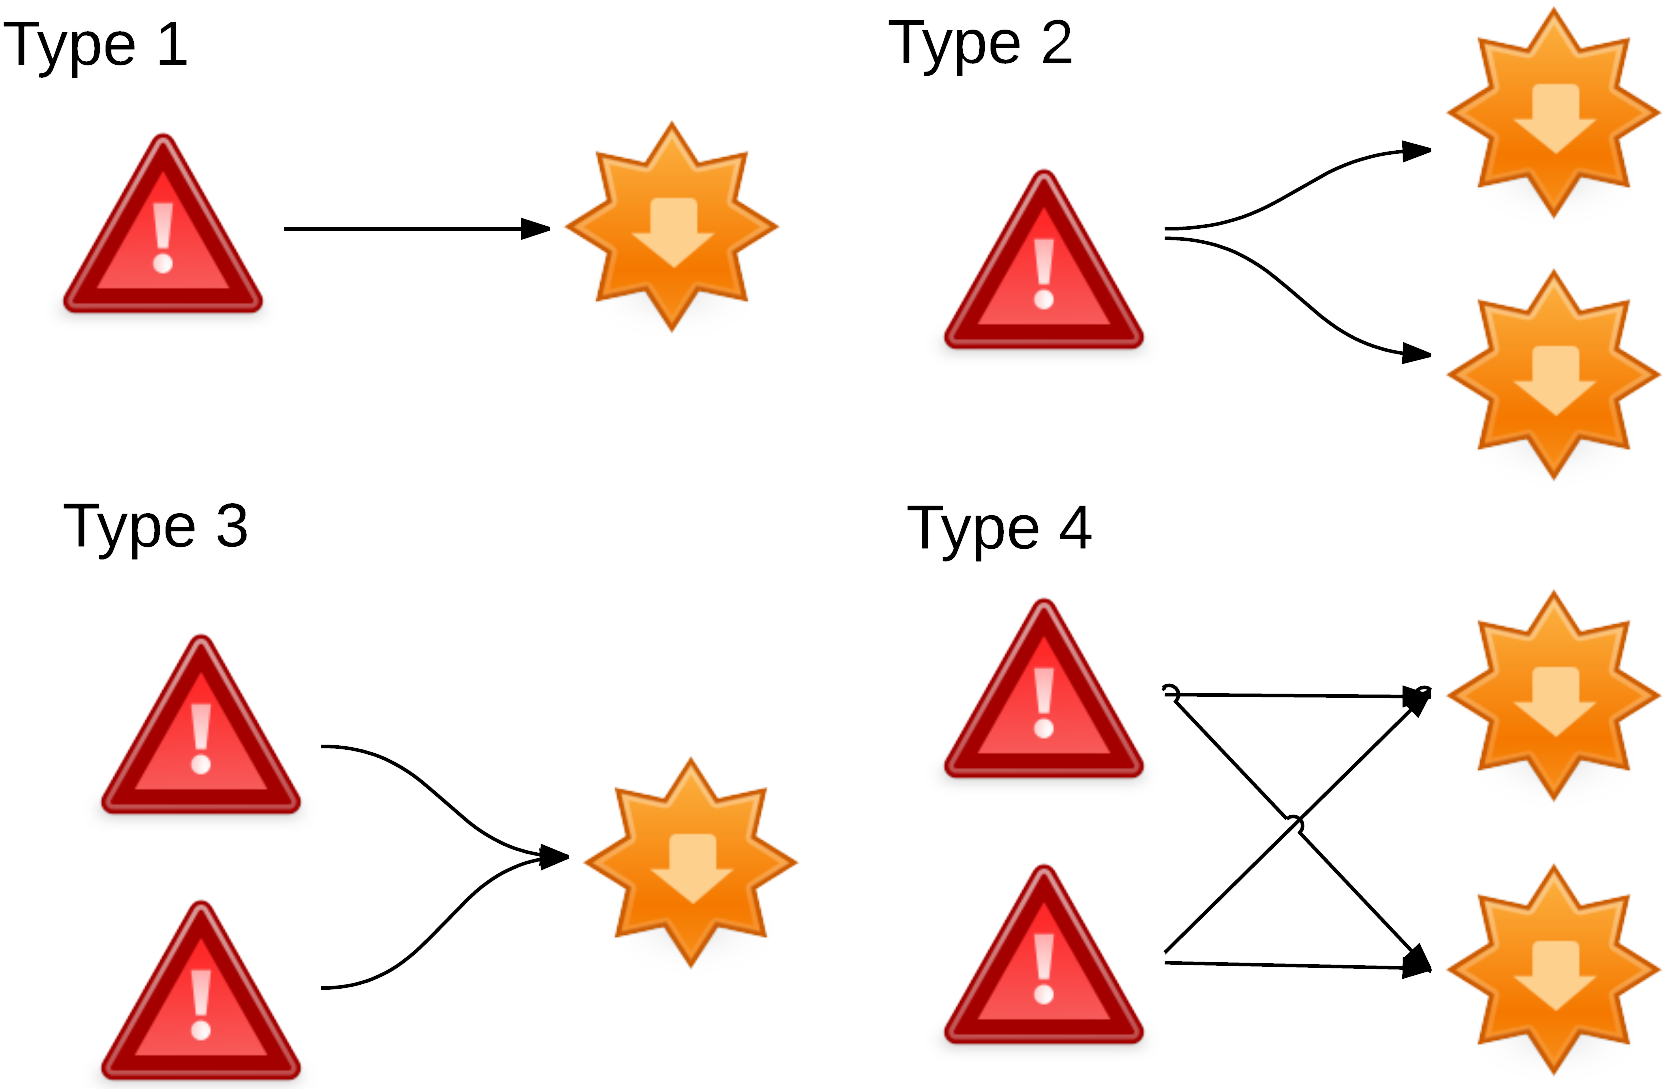
\includegraphics[scale=0.8]{media/bug-taxo.png}
    \caption{Proposed Taxonomy of Bugs
    \label{fig:bug-taxo}}
\end{figure}


The first and second types are the ones we intuitively know
about. Type 1 refers to a bug being fixed in one single location
(i.e., one file), while Type 2 refers to bugs being fixed in more
than one location. In Figure 2, only two locations are shown
for the sake of clarity, but many more locations could be
involved in the fix of a bug. Type 3 refers to multiple bugs that
are fixed in the exact same location. Type 4 is an extension of
Type 3, where multiple bugs are resolved by modifying the
same set of locations. Note that Type 3 and Type 4 bugs are
not duplicates, they may occur when different features of the
system fail due to the same root causes (faults).
We conjecture that knowing the proportions of each type
of bugs in a system may provide insight into the quality of the
system. Knowing, for example, that in a given system the
proportion of Type 2 and 4 bugs is high may be an indication
of poor system quality since many fixes are needed to address
these bugs. In addition, the existence of a high number of
Types 3 and 4 bugs calls for techniques that can effectively
find bug reports related to an incoming bug during triaging.
This is similar to the many studies that exist on detection of
duplicates (e.g., \cite{Runeson2007,Sun2010,Nguyen2012}), except that we are not looking for
duplicates but for related bugs (bugs that are due to failures of
different features of the system, caused by the same faults). To
our knowledge, there is no study that exmpirically examines
bug data with these types in mind, which is the main objective
of this section. More particularly, we are interested in the
following research questions:

\begin{itemize}
	\item RQ1: What are the proportions of different types of bugs?
	\item RQ2: How complex is each type of bugs?
	\item RQ3: How fast are these types of bugs fixed?
\end{itemize}


\section{Study Setup}

Figure \ref{fig:bug-taxo-flow} illustrates our data collection and analysis
process that we present here and discuss in more detail in the
following subsections. First, we extract the raw data from the
two bug report management systems used in this study
(Bugzilla and Jira). Second, we extract the fix to the bugs
from the source code version control system of Netbeans and
Apache (Maven and Git).

\begin{figure}[h!]
  \centering
    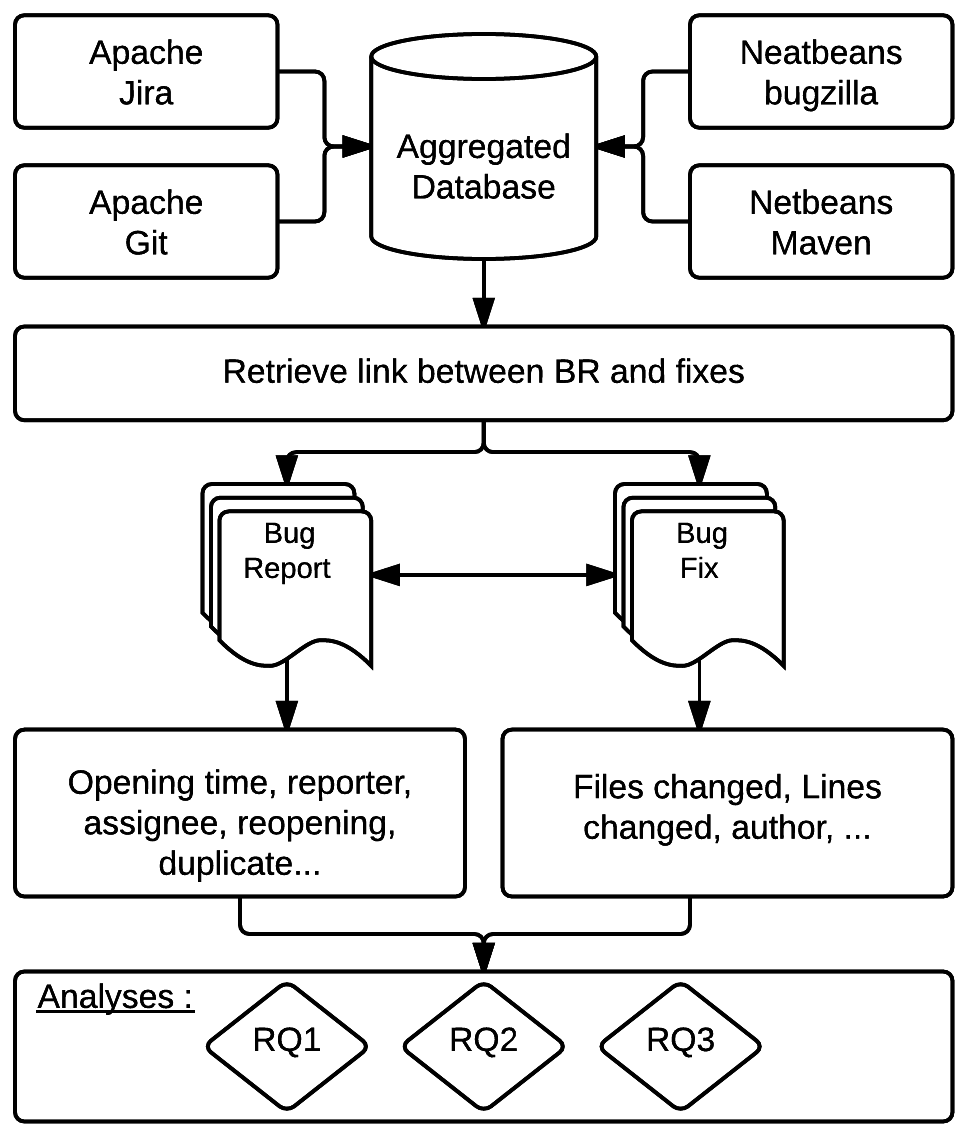
\includegraphics{media/bug-taxo-flow.png}
    \caption{Data collection and analysis process of the study
    \label{fig:bug-taxo-flow}}
\end{figure}


The extracted data is
consolidated in one database where we associate each bug
report to its fix. We mine relevant characteristics of BRs and
their fixes such as opening time, number of comments,
number of times the BR is reopened, number of changesets
for BR and the number of files changed and lines modified
for fixes or patch. Finally, we analyze these characteristics to
answer the aforementioned research questions (RQ).


\section{Study Design}

We describe the design of our study by first stating the
research questions, and then explaining the variables, and
analysis methods we used to answer these questions. We
formulate three research questions (RQs) with the ultimate
goal to improve our understanding of each bug type. We
focus, however, on Types 2 and 4. This is because these bugs
require multiple fixes. They are therefore expected to be more
complex.
The objective of the first research question is to analyze
the proportion of each type of bugs. The remaining two
questions address the complexity of the bugs and the bug
fixing duration according to the type of bugs.
1)

\subsection{RQ 1: What are the proportions of different types of bugs?}

The answer to this question provides insight into the
distribution of bugs according to their type with a focus on
Type 2 and 4 bugs. As discussed ealier, knowing, for
example, that bugs of Type 2 and 4 are the most predominant
ones suggests that we need to investigate techniques to help
detect whether an incoming bug is of Types 2 and 4 by
examining historical data. Similarly, if we can automatically
identify a bug that is related to another one that has been fixed
then we can reuse the results of reproducing the first bug in
reproducing the second one.

{\bf Hypothesis}: To answer this question, we analyze whether
Type 2 and 4 bugs are predominant in the studied systems, by
testing the null hypothesis:

\begin{itemize}
	\item $H_{01A}$ : The proportion of Types 2 and 4 does not
change significantly across the studied systems
\end{itemize}


We test this hypothesis by observing both a “global”
(across systems) and a “local” predominance (per system) of
the different types of bugs. We must observe these two
aspects to ensure that the predominance of a particular type of
bug is not circumstantial (in few given systems only) but is
also not due to some other, unknown factors (in all systems
but not in a particular system).

{\bf Variables}: We use as variables the amount of resolved/fixed
bugs of each type (1, 2, 3 and 4) that are linked to a fix
(commit). As mentioned earlier, duplicate bugs are excluded.
These are marked as resolved/duplicate in our dataset.

{\bf Analysis Method}: We answer RQ1 in two steps. The first
step is to use descriptive statistics; we compute the ratio of
Types 2 and 4 bugs and the ratio of Types 1 and 3 bugs to the
total number of bugs in the dataset. This shows the
importance of Types 2 and 4 bugs compared to Types 1 and 3
bugs.

In the second step, we compare the proportions of the
different types of bugs with respect to the system where the
bugs were found. We build the contingency table with these
two qualitative variables (the type and studied system) and
test the null hypothesis H 01A to assess whether the proportion
of a particular type of bugs is related to a specific system or
not.

We use the Pearson's chi-squared test to reject the null
hypothesis $H_{01A}$ . Pearson’s chi-squared independence test is
used to analyze the relationship between two qualitative data,
in our study the type bugs and the studied system. The results
of Pearson’s chi-squared independence test are considered
statistically significant at $\alpha$ = 0.05. If p-value $\le$ 0.05, we
reject the null hypothesis $H_{01A}$ and conclude that the
proportion of types 3 and 4 bugs is different from the
proportion of type 1 and 2 bugs for each system.

\subsection{RQ 2: How complex is each type of bugs?}

We address the relation between Types 2 and 4 bugs and
the complexity of the bugs in terms of severity, duplicate and
reopened.We analyze whether Types 2 and 4 bugs are more
complex to handle than Types 1 and 3 bugs, by testing the
null hypotheses:

\begin{itemize}
 \item  $H_{02S}$ : The severity of Types 2 and 4 bugs is not
significantly different from the severity of Types 1 and 3
 \item  $H_{02D}$ : Types 2 and 4 bugs are not significantly more
likely to get duplicated than Types 1 and 3.
 \item  $H_{02R}$ : Type 2 and 4 bugs are not significantly more
likely to get reopened than Types 1 and 3.
\end{itemize}

{\bf Variables}: We use as independent variables for the
hypotheses $H_{02S}$ , $H_{02D}$ , $H_{02R}$ the bug type (if the bug is from
Types 2 and 4 or if it is from Types 1 and 3). For $H_{02S}$  we use
the severity as dependent variable to assess the relationship
between the bug severity and the bug type. For $H_{02D}$
(respectively $H_{02R}$) we use a dummy variable duplicated
(reopened) to assess if a bug has been duplicated (reopened)
at least once or not. This will be used to assess the
relationship between the type of the bugs and the fact that the
bug is more likely to be reopened or duplicated.

{\bf Analysis Method}: For each hypothesis, we build a
contingency table with the qualitative variables type of bugs
(2 and 4 or 1and 3) and the dependent variable duplicated
(respectively reopened) and the severity variable.

We use the Pearson’s chi-squared test to reject the null
hypothesis $H_{02D}$ (respectively $H_{02R}$ ) and $H_{02S}$. The results of
Pearson’s chi-squared independence test are considered
statistically significant at $\alpha$ = 0.05. If a p-value $\le$ 0.05, we
reject the null hypothesis  $H_{02D}$ (respectively $H_{02R}$) and
conclude the fact that the bug is more likely to be duplicated
(respectively reopened) is related to the type of the bug and
we reject $H_{02S}$ and conclude that the severity level of the bug
is related to the bug type.

\subsection{RQ 3 : How fast are these types of bugs fixed ?}

In this question, we study the relation between the
different types of bugs and the fixing time. We are interested
in evaluating whether developers take more time to fix Types
2 and 4 bugs than Type 1 and 3, by testing the null hypothesis:

\begin{itemize}
	\item $H_{03}$ : There is no statistically-significant difference
between the duration of fixing periods for Types 2 and
4 bugs and that of Types 1 and 3 bugs.
\end{itemize}


{\bf Variables}: To compare the bug fixing time with respect to
their type, we use as independent variable the type Ti of a
bug Bi, to distinguish between Types 1 and 3 bugs and Types
2 and 4 bugs. We consider as dependent variable the fixing
time, FTi, of the bug Bi. We compute the fixing time FTi of a
bug Bi. The fixing time FTi is the time between when the bug
is submitted to when it is closed/fixed.

{\bf Analysis Method}: We compute the (non-parametric) Mann-
Whitney test to compare the BR fixing time with respect to
the BR type and analyze whether the difference in the average
fixing time is statistically significant. We use the Mann-
Whitney test because, as a non-parametric test, it does not
make any assumption on the underlying distributions. We
analyze the results of the test to assess the null hypothesis
$H_{03}$ . The result is considered as statistically significant at $\alpha$ =
0.05. Therefore, if p-value $\le$ 0.05, we reject the null
hypothesis H 03 and conclude that the average fixing time of
Types 1 and 3 bugs is significantly different from the average
fixing time of Types 2 and 4 bugs.

\section{Study result and discussion}

In this section, we report on the results of the analyses we
performed to answer our research questions. We then dedicate
a section to discussing the results.

\subsection{RQ 1 : What are the proportions of different types of
bugs?}

Figure \ref{fig:bug-taxo-rq1} shows the percentage of the different types of
bugs. As shown in the figure, we found that 65\% of the bugs
are from Types 2 and 4. This shows the predominance of this
type of bugs in all the studied systems. Figure 5 shows the
repartition per dataset. We can see that Netbeans and Apache
have 66\% and 64\% bugs of Type 1and 3, respectively. To
ensure that this observation is not related to a particular
system, we perform Pearson’s chi-squared test across the
studied systems. Table \ref{tab:bug-taxo-rq1} shows the contingency table for the
studied systems and the result of Pearson’s chi-squared test.
The results show that there is statistically significant
difference between the proportions of the different types of
bugs.

\begin{table}[h!]
\centering
\begin{tabular}{c|c|c|c}
{System} & {Type 1 and 3} & {Type 2 and 4} & {Pearson’s chisquared p-value}        \\  \hline \hline
Apache       & 4910               & 8626               & \multirow{2}{*}{p-value \textless 0,0001} \\ \cline{1-3}
Netbeans     & 9050               & 17586              & \\ \hline \hline
\end{tabular}
\caption{Contingency table and Pearson's chi-squared tests\label{tab:bug-taxo-rq1}}
\end{table}

\begin{figure}[h!]
  \centering
    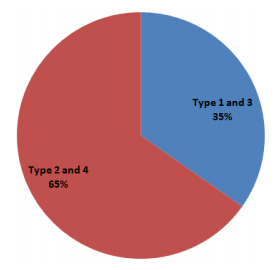
\includegraphics[scale=0.7]{media/bug-taxo-rq1.png}
    \caption{Proportions of different types of bugs
    \label{fig:bug-taxo-rq1}}
\end{figure}

Table \ref{tab:bug-taxo-rq1-prop} shows the number of bugs for each type of bugs
and the percentage of each type of bugs. We can see that
Types 3 and 4 bugs represent 28.33\% and 61.21\% of the total
of bugs, respectively. Types 1 and 2 represent only 6.78\% and
3.74\%. Together, Types 3 and 4 bugs represent almost 90\%
of the total number of bugs linked to a commit.

\begin{table}[h!]
\centering

\begin{tabular}{c|c|c|c|c|c}
Datasets                  & T1        & T2       & T3        & T4        & Total                  \\ \hline \hline
\multirow{2}{*}{Netbeans} & 776       & 240      & 8372      & 17366     & \multirow{2}{*}{26754} \\
                          & (2.90\%)  & (0.90\%) & (31.29\%) & (64.91\%) &                        \\ \hline
Apache                    & 1968      & 1248     & 3101      & 7422      & \multirow{2}{*}{13739} \\
                          & (14.32\%) & (9.08\%) & (22.57\%) & (54.02\%) &                        \\ \hline
\multirow{2}{*}{Total}    & 2744      & 1488     & 11473     & 24788     & \multirow{2}{*}{40493} \\
                          & (6.78\%)  & (3.74\%) & (28.33\%) & (61.21\%) & \\ \hline \hline
\end{tabular}
\caption{Proportion of bug types in amount and percentage}
\label{tab:bug-taxo-rq1-prop}
\end{table}


\noindent\fbox{%
    \parbox{\textwidth}{%
      We can thus reject the null hypothesis $H_{01A}$ and
conclude that there is a predominance of Types 2 and
4 bugs in all studied systems and this observation is
not related to a specific system.
    }%
}

\subsection{RQ 2 : How complex is each type of bugs?}

Figure \ref{fig:bug-taxo-rq2-prop-apache} and \ref{fig:bug-taxo-rq2-prop-netbeans} show the proportion of each bug type with
respect to their severity for each dataset. Table V shows the
proportion of each bug type with repect to their severity and
dataset. For Netbeans, the bugs we examined in our dataset
are either labeled as Blocker or Normal (despite the fact that
Netbeans uses Bugzilla that supports all the severity levels
presented in the previous section).

\begin{figure}[h!]
  \centering
    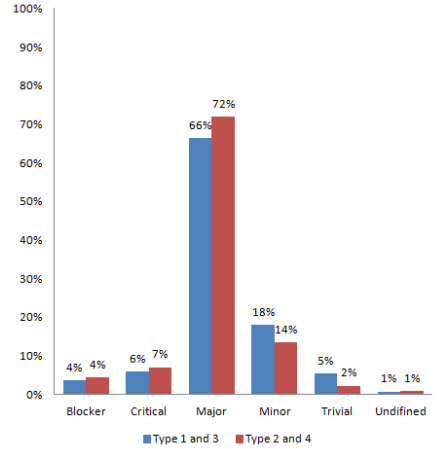
\includegraphics[scale=0.6]{media/bug-taxo-rq2-prop-apache.png}
    \caption{Proportions of Types 1 and 3 versus Types 2 and 4 with respct to their severity in the Apache dataset.
    \label{fig:bug-taxo-rq2-prop-apache}}
\end{figure}

\begin{figure}[h!]
  \centering
    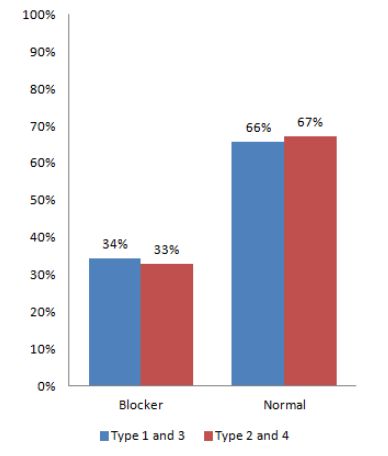
\includegraphics[scale=0.6]{media/bug-taxo-rq2-prop-netbeans.png}
    \caption{Proportions of Types 1 and 3 versus Types 2 and 4 with respct to their severity in the Netbeans dataset.
    \label{fig:bug-taxo-rq2-prop-netbeans}}
\end{figure}

For the Apache dataset, the severity levels range from
Blocker to Trivial as shown in Figure \ref{fig:bug-taxo-rq2-prop-apache}. Figure \ref{fig:bug-taxo-rq2-prop-netbeans} shows that
in Netbeans around 67\% of Types 2 and 4 bugs are normal.
The same holds for Types 1 and 3 bugs (66\% are considered
of normal severity). This indicates that most Types 2 and 4
bugs and Types 1 and 3 bugs are not critical in the Netbeans
dataset. For the Apache dataset, the results indicate that the
majority of the bugs are considered of major severity (66\%
for Types 1 and 3 and 72\% for Types 2 and 4). It is
challenging to understand the discrepancy between the two
datasets partly because of the way the severity is assigned to
BRs.

Table \ref{tab:bug-taxo-rq2-chi} shows the result of the Pearson chi-squared tests
for the $H_{02S}$, $H_{02D}$ and $H_{02R}$ hypotheses.

\begin{table}[h!]
\centering
\begin{tabular}{c|c|c}
System                    & Factor     & \begin{tabular}[c]{@{}c@{}}Pearson’s chisquared\\ p-value\end{tabular} \\ \hline \hline
\multirow{3}{*}{Apache}   & Severity   & p-value \textless 0.005                                                \\
                          & Reopened   & p-value \textless 0.005                                                \\
                          & Duplicated & p-value \textless 0.005                                                \\ \hline \hline
\multirow{3}{*}{Netbeans} & Severity   & p-value \textless 0.005                                                \\
                          & Reopened   & p-value \textless 0.005                                                \\
                          & Duplicated & p-value \textless 0.005  \\  \hline \hline
\end{tabular}

\caption{Pearson's chi squared p-values for the severity, the reopen and the duplicate factor with respect to a dataset}
\label{tab:bug-taxo-rq2-chi}
\end{table}

\noindent\fbox{%
    \parbox{\textwidth}{%
      According to the results of the test (p-value < 0.005),
we reject the null hypothesis $H_{02S}$ and conclude that
there is a significant difference between the severity of
Types 1 and 3 bugs and the severity of Types 2 and 4
bugs.
    }%
}

\begin{table}[h!]
\centering
\begin{tabular}{c|c|c|c|c}
Severity                  & T1      & T2      & T3      & T4      \\
\hline \hline
\multicolumn{5}{c}{Netbeans}                                      \\ \hline
\multirow{2}{*}{Blocker}  & 340     & 109     & 2850    & 5687    \\
                          & 43.81\% & 45.42\% & 34.04\% & 32.75\% \\ \hline
\multirow{2}{*}{Normal}   & 436     & 131     & 5522    & 11678   \\
                          & 56.19\% & 54.58\% & 65.96\% & 67.25\% \\
                          \hline
\multirow{2}{*}{Total}    & 776     & 240     & 8372    & 17365   \\
                          & 100\%   & 100\%   & 100\%   & 100\%   \\
\hline \hline
\multicolumn{5}{c}{Apache}                                        \\ \hline
\multirow{2}{*}{Blocker}  & 68      & 53      & 115     & 329     \\
                          & 3.46\%  & 4.25\%  & 3.71\%  & 4.43\%  \\
                          \hline
\multirow{2}{*}{Critical} & 84      & 44      & 213     & 565     \\
                          & 4.27\%  & 3.53\%  & 6.87\%  & 7.61\%  \\
                          \hline
\multirow{2}{*}{Major}    & 1245    & 811     & 2096    & 5427    \\
                          & 63.26\% & 64.98\% & 67.59\% & 73.12\% \\
                          \hline
\multirow{2}{*}{Minor}    & 408     & 276     & 501     & 899     \\
                          & 20.73\% & 22.12\% & 16.16\% & 12.11\% \\
                          \hline
\multirow{2}{*}{Trivial}  & 113     & 31      & 159     & 161     \\
                          & 5.74\%  & 2.48\%  & 5.13\%  & 2.17\%  \\
                          \hline
\multirow{2}{*}{Total}    & 1918    & 1215    & 3084    & 7381    \\
                          & 100\%   & 100\%   & 100\%   & 100\%  \\
\hline \hline
\end{tabular}
\caption{Proportion of each bug type with respect to severity.}
\label{tab:bug-taxo-rq2-severity}
\end{table}

Table \ref{tab:bug-taxo-rq2-dup} shows the occurrences of duplicate and reopened
bugs with respect to their bug type in each dataset. In
Netbeans, the proportion of Type 1 bugs that are marked as
source of duplicate is 6.06\%, 4.59\% for Type 2 bugs, 5.09\%
for Type 3 bugs and 5.87\% for Type 4 bugs with a total of
1503 bugs over 26754 (5.62\%). In Apache, the proportion of
Type 1 bug marked a source of a duplicate is 2.59\% and
2.24\%, 1.61\% and 2.91\% for Types 2, 3 and 4, respectively.

\begin{table}[h!]
\centering
\begin{tabular}{c|c|c|c|c|c}
Type                   & T1     & T2     & T3     & T4     & Total  \\ \hline \hline
\multicolumn{6}{c}{Netbeans}                                      \\ \hline \hline
\multirow{2}{*}{Dup.}  & 6.06\% & 4.59\% & 5.09\% & 5.87\% & 5.62\% \\
                       & (47)   & (11)   & (426)  & (1019) & (1503) \\ \hline
\multirow{2}{*}{Reop.} & 4.38\% & 7.08\% & 4.81\% & 7.09\% & 6.30\% \\
                       & (34)   & (17)   & (403)  & (1231) & (1685) \\ \hline
\multicolumn{6}{c}{Apache}                                        \\ \hline \hline
\multirow{2}{*}{Dup}   & 2.59\% & 2.24\% & 1.61\% & 2.91\% & 2.51\% \\ \
                       & (51)   & (28)   & (50)   & (216)  & (345)  \\ \hline
\multirow{2}{*}{Reop}  & 5.59\% & 6.49\% & 3.10\% & 6.90\% & 5.82\% \\
                       & (110)  & (81)   & (96)   & (512)  & (799)  \\ \hline
\multicolumn{6}{c}{Total}                                         \\ \hline \hline
\multirow{2}{*}{Dup}   & 3.57\% & 2.62\% & 4.15\% & 4.98\% & 4.56\% \\
                       & (98)   & (39)   & (476)  & (1235) & (1848) \\ \hline
\multirow{2}{*}{Reop}  & 5.25\% & 6.59\% & 4.35\% & 7.03\% & 6.13\% \\
                       & (144)  & (98)   & (499)  & (1743) & (2484) \\ \hline
\end{tabular}
\caption{Percentage and occurences of bugs duplicated by other bufs and reopenned with respect to their bug type and dataset.}
\label{tab:bug-taxo-rq2-dup}
\end{table}

Second, we analyze the reopened bugs to see the link
between the reopening and the type of bugs. We perform
Pearson’s chi-squared test to reject the null hypothesis $H_{02R}$.

\noindent\fbox{%
    \parbox{\textwidth}{%
      According to the results of the test (p-value <
0.005), we reject the null hypothesis $H_{02R}$ and
conclude that there is a significant relationship
between the reopening of a bug and its type.
    }%
}

Third, we analyze the duplicated bugs to see if there is a
link between the bug type and the fact duplication. We
perform Pearson’s chi-squared test to reject the null
hypothesis $H_{02D}$.

\noindent\fbox{%
    \parbox{\textwidth}{%
      According to the results of the test (p-value <
0.005), we reject the null hypothesis $H_{02D}$ and
conclude that there is a significant relationship
between the duplication of a bug and its type.
    }%
}

\subsection{RQ 3 : How fast are these types of bugs fixed ?}

Figure \ref{fig:bug-taxo-rq3} shows the fixing time for Types 1 and 3 versus
Types 2 and 4 for Netbeans and the Apache Software
Foundation. In Netbeans, 98.96 and 137.05 days are required
to fix Types 1 and 3 and Types 2 and 4, respectively. In
Apache, 55.76 and 85.48 days are required to fix Types 1 and
3 and Types 2 and 4, respectively.


\begin{figure}[h!]
  \centering
    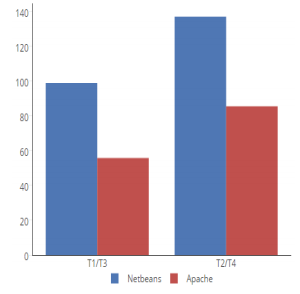
\includegraphics[scale=0.8]{media/bug-taxo-rq3.png}
    \caption{Fixing time of Types 1 and 3 versus fixing time of Types 2 and 4.
    \label{fig:bug-taxo-rq3}}
\end{figure}

Table \ref{tab:bug-taxo-rq3} shows the average fixing time of bugs with respect
to their bug type in each dataset.

\begin{table}[h!]
\centering
\begin{tabular}{c|c|c|c|c|c}
Dataset  & T1    & T2     & T3     & T4     & Average \\ \hline \hline
Netbeans & 97.66 & 117.42 & 100.26 & 156.67 & 118.00  \\ \hline
Apache   & 73.48 & 118.12 & 38.04  & 52.83  & 70.62   \\ \hline
Total    & 85.57 & 117.77 & 69.15  & 104.75 & 94.31  \\ \hline \hline
\end{tabular}
\caption{Average fixing time with respect to bug type
    \label{tab:bug-taxo-rq3}}
\end{table}

We analyze the difference in the fixing time of bugs with
respect to their bug type by conducting a Mann-Whitney test
to assess $H03$.The results show that the difference between
the fixing time of Types 2 and 4 and Types 1 and 3 is
statistically significant (p-value < 0,005).

\noindent\fbox{%
    \parbox{\textwidth}{%
      Therefore, we can reject the null hypothesis $H03$ and
conclude that the fixing of Types 2 and 4 bugs takes
more time than the fixing of Types 1 and 3 bugs.
    }%
}

\subsubsection{Dicussion}

{\bf Repartition of bug types}: One important finding of this
study is that there is significantly more Types 2 and 4 bugs
than Types 1 and 3 in all studied systems. Moreover, this
observation is not system-specific. The traditional one-bug/
one-fault way of thinking about bugs only accounts for 35\%
of the bugs. We believe that, recent triaging algorithms
\cite{Jalbert2008,Jeong2009,Khomh2011a,Tamrawi2011a} can benefit from these findings by developing
techniques that can detect Type 2 and 4 bugs. This would
result in better performance in terms of reducing the cost,
time and efforts required by the developers in the bug fixing
process.

{\bf Severity of bugs}: We discussed the severity and the
complexity of a bug in terms of its likelihood to be reopened
or marked as duplicate (RQ2). Although clear guidelines exist
on how to assign the severity of a bug, it remains a manual
process done by the bug reporter. In addition, previous
studies, notably those by Khomh et al. \cite{Khomh2011a}, showed that severity is not a consistent/trustworthy characteristic of a BR,
which lead to he emergence of studies for predicting the
severity of bugs (e.g., \cite{Lamkanfi2010,Lamkanfi2011,Tian2012}). Nevertheless, we
discovered that there is a significant difference between the
severities of Types 1 and 3 compared to Types 2 and 4.

{\bf Complexity of bugs}: At the complexity level, we use the
number of times a bug is reopened as a measure of
complexity. Indeed, if a developer is confident enough in
his/her fix to close the bug and that the bug gets reopened it
means that the developer missed some dependencies of the
said bug or did not foresee the consequences of the fix.
We found that there is a significant relationship between
the number of reopenings and type of a bug. In other words,
there is a significant relationship between the complexity and
the type of a given bug. In our datasets, Types 1 and 3 bugs
are reopened in 1.88\% of the cases, while Types 2 and 4 are
reopened in 5.73\%. Assuming that the reopening is a
representative metric for the complexity of bug, Types 2 and
4 are three times more complex than Types 1 and 3. Finally, if
we consider multiple reopenings, Types 2 and 4 account for
almost 80\% of the bugs that reopened more than once and
more than 96\% of the bug opened more than twice.
While current approaches aiming to predict which bug
will be reopen use the amount of modified files \cite{Shihab2010,Zimmermann2012,Lo2013}, we
believe that they can be improved by taking into account the type of a the bug. For example, if we can detect that an
incoming bug if of Type 2 or 4 then it is more likely to
reopened than a bug of Type 1 or 3. Similarly, approaches
aiming to predict the files in which a given bug should be
fixed could be categorized and improved by knowking the
bug type in advance \cite{Zhou2012,Kim2013a}.

{\bf Impact of a bug}: To measure the impact of bugs in end-users
and developers, we use the number of times a bug is
duplicated. This is because if a bug has many duplicates, it
means that a large number of users have experienced and a
large number of developers are blocked the failure.
We found that there is a significant relationship between
the bug type and the fact that it gets duplicated. Types 1 and 3
bugs are duplicated in 1.41\% of the cases while Types 2 and 4
are duplicated in 3.14\%. Assuming that the amount of
duplication is an accurate metric for the impact of bug, Types
2 and 4 have more than two times bigger impact than Types 1
and 3. Similarly to reopening, if we consider multiple
duplication, Types 2 and 4 account for 75\% of the bugs that
get duplicated more than once and more than 80\% of the bugs
that get duplicated more than twice.
We believe that approaches targeting the identification of
duplicates \cite{Bettenburg2008a,Jalbert2008,Sun2010,Tian2012a}  could leverage this taxonomy to
achieve even better performances in terms of recall and
precision.

{\bf Fixing time}: Our third research question aimed to determine
if the type of a bug impacts its fixing time. Not only we found
that the type of a bug does significantly impact its fixing time,
but we also found that, in average Types 2 and 4, stay open
111.26 days while Types 1 and 3 last for 77.36 days. Types 2
and 4 are 1.4 time longer to fix than Types 1 and 3.We
therefore believe that, approaches aiming to predict the fixing
time of a bug (e.g., \cite{Panjer2007,Bhattacharya2011,Zhang2013}) can highly benefit from
accurately predicting the type of a bug and thereforebetter
plan the required man-power to fix the bug.
In summary, Types 2 and 4 account for 65\% of the bugs
and they are more complex, have a bigger impact and take
longer to be fixed than Types 1 and 3 while being equivalent
in terms of severity.

Our taxonomy aimed to analyse: (1) the
proportion of each type of bugs; (2) the complexity of each
type in terms of severity, reopening and duplication; (3) the
required time to fix a bug depending on its type. The key
findings are:
\begin{itemize}
  \item Types 2 and 4 account for 65\% of the bugs.
  \item Types 2 and 4 have a similar severity compared to
Types 1 and 3.
  \item Types 2 and 4 are more complex (reopening) and have
a bigger impact (duplicate) than Types 1 and 3.
  \item It takes more time to fix Types 2 and 4 than Types 1
and 3.
\end{itemize}

Our taxonomy and results can be built upon in order to classify
past and new researches in several active areas such as bug
reproduction and triaging, prediction of reopening,
duplication, severity, files to fix and fixing time. Moreover, if
one could predict the type of a bug at submission time, all
these areas could be improved.

